%%%%%%%%%%%%%%%%%%%%%%% file template.tex %%%%%%%%%%%%%%%%%%%%%%%%%
%
% This is a general template file for the LaTeX package SVJour3
% for Springer journals.          Springer Heidelberg 2010/09/16
%
% Copy it to a new file with a new name and use it as the basis
% for your article. Delete % signs as needed.
%
% This template includes a few options for different layouts and
% content for various journals. Please consult a previous issue of
% your journal as needed.
%
%%%%%%%%%%%%%%%%%%%%%%%%%%%%%%%%%%%%%%%%%%%%%%%%%%%%%%%%%%%%%%%%%%%
%
% First comes an example EPS file -- just ignore it and
% proceed on the \documentclass line
% your LaTeX will extract the file if required
\begin{filecontents*}{example.eps}
%!PS-Adobe-3.0 EPSF-3.0
%%BoundingBox: 19 19 221 221
%%CreationDate: Mon Sep 29 1997
%%Creator: programmed by hand (JK)
%%EndComments
gsave
newpath
  20 20 moveto
  20 220 lineto
  220 220 lineto
  220 20 lineto
closepath
2 setlinewidth
gsave
  .4 setgray fill
grestore
stroke
grestore
\end{filecontents*}
%
\RequirePackage{fix-cm}
%
%\documentclass{svjour3}                     % onecolumn (standard format)
%\documentclass[smallcondensed]{svjour3}     % onecolumn (ditto)
\documentclass[smallextended]{svjour3}       % onecolumn (second format)
%\documentclass[twocolumn]{svjour3}          % twocolumn
%
\smartqed  % flush right qed marks, e.g. at end of proof
%
\usepackage{graphicx}
%\usepackage{todonotes}
\usepackage[colorinlistoftodos]{todonotes}
\newcommand{\Dtodo}{\todo[inline, color=red!50!]}
\newcommand{\Ctodo}{\todo[inline, color=blue!50!]}

%Replacement for the above after the style Bas used
% Comments
\newcounter{comment}
\newcommand{\comment}[2][]{%
% initials of the author (optional) + note in the margin
\refstepcounter{comment}%
{%
\todo[inline, color={red!50},size=\small]{%
\textbf{\footnotesize [\uppercase{#1}\thecomment]:}~#2}%
}}

% Insert the name of "your journal" with
\journalname{Journal of Computer-Aided Molecular Design}
\begin{document}

\title{Blind prediction of cyclohexane-water distribution coefficients from the SAMPL5 challenge}
\titlerunning{SAMPL5 distribution coefficients}
\thanks{We appreciate financial support from the National Institutes of Health (1R01GM108889-01) and the National Science Foundation (CHE 1352608), and computing support from the UCI GreenPlanet cluster, supported in part by NSF Grant CHE-0840513. 
This work was made possible in part by NIH grant U01 GM111528. The contents of this paper are solely the responsibility of the authors and do not necessarily represent the official views of the NIH.
M.K.G. has an equity interest in and is a cofounder and scientiÞc advisor of VeraChem LLC. } % Is this where this belongs?

% The Thanks isn't printing, so I also included the financial support in the acknowledgements at the bottom of the paper. 

\author{Caitlin C. Bannan         \and
        Kalistyn H. Burley \and
        Michael Chiu \and
        Michael R. Shirts \and
        Michael K. Gilson \and
        David L. Mobley
}
\institute{C. C. Bannan \at Department of Chemistry, University of California, Irvine
	\and
	K. H. Burley \at Department of Pharmaceutical Sciences, University of California, Irvine
	\and
	M. Chiu \at Qualcomm Institute, University of California, San Diego
	\and
	M. R. Shirts \at Chemical and Biological Engineering, University of Colorado, Boulder
	\and
	M. K. Gilson \at Skaggs School of Pharmacy and Pharmaceutical Sciences, University of California, San Diego 
	\and
	D. L. Mobley \at Department of Chemistry and Department of Pharmaceutical Sciences, University of California, Irvine\\
		147 Bison Modular, Irvine, CA 92697
              Tel.: +949-824-6383\\
              Fax: +949-824-2949\\
              \email{dmobley@mobleylab.org} }          

\date{Received: date / Accepted: date}
% The correct dates will be entered by the editor
\maketitle

\begin{abstract}

In the recent SAMPL5 challenge, participants submitted predictions for cyclohexane/water distribution coefficients for a set of 53 small molecules. 
Distribution coefficients ($\log D$) replace the hydration free energies that were a central part of the past five SAMPL challenges.
A wide variety of computational methods were represented by the 76 submissions from 18 participating groups. 
Here, we analyze submissions by a variety of error metrics and provide details for a number of reference calculations we performed. 
As in the SAMPL4 challenge, we assessed the ability of participants to evaluate not just their statistical uncertainty, but their model uncertainty -- how well they can predict the magnitude of their model or force field error for specific predictions. 
Unfortunately, this remains an area where prediction and analysis need improvement. 
In SAMPL4 the top performing submissions achieved a root-mean-squared error (RMSE) around 1.5 kcal/mol. 
If we anticipate accuracy in $\log D$ predictions to be similar to the hydration free energy predictions in SAMPL4, the expected error here would be around 1.54 log units. 
Only a few submissions had an RMSE below 2.5 log units in their predicted $\log D$ values. 
However, distribution coefficients introduced complexities not present in past SAMPL challenges, including tautomer enumeration, that are likely to be important in predicting biomolecular properties of interest to drug discovery, therefore some decrease in accuracy would be expected.
Overall, the SAMPL5 distribution coefficient challenge provided great insight into the importance of modeling a variety of physical effects. 
We believe these types of measurements will be a promising source of data for future blind challenges, especially in view of the relatively straightforward nature of the experiments and the level of insight provided. 

\keywords{SAMPL \and distribution coefficient \and blind challenge \and free energy \and alchemical \and molecular simulation } 
\end{abstract}

\section{Introduction}
\label{intro}

This year's Statistical Assessment of Modeling of Proteins and Ligand (SAMPL) challenge focuses on prediction of cyclohexane-water distribution coefficients. 
The inclusion of distribution coefficients replaces the previous focus on hydration free energies which was a fixture of the past five challenges (SAMPL0-4)  \cite{Mobley:2014gu,Geballe:2012fc,Geballe:2010jr,Klimovich:2010jm,Mobley:2009iu,Mobley:2012jwa,Nicholls:2008cx}.
Due to a lack of ongoing experimental work to generate new data, hydration free energies are no longer a practical property to include in blind challenges. 
It has become increasingly difficult to find unpublished or obscure hydration free energies and therefore impossible to design a challenge focusing on target compounds, functional groups or chemical classes. 
But this type of data is extremely valuable --- the past SAMPL challenges have driven real improvements in a variety of methods for calculating hydration free energies  \cite{Mobley:2014gu} --- so we sought to include a similar physical property in SAMPL5. 
The organizers of SAMPL5 settled on cyclohexane-water distribution coefficients, and thanks to a partnership with Genentech, this led to a series of measurements on drug-like compounds, discussed in detail in this issue  \cite{Rustenburg:sampl5}.
The experimental measurements are also straightforward enough that future distribution coefficient challenges can be deliberately designed to focus on issues that merit attention to move the field forward.

Partition and distribution coefficients are important physical properties  \cite{Leo:1971wu,Young:2011gs} which can provide a valuable opportunity for testing computational methods and molecular models. 
Distribution coefficients describe how all forms of a solute distributes itself across two immiscible solvents. 
In this case,
\begin{equation}
D = \frac{\sum_i [X_i]_{cyc}}{\sum_i [X_i]_{aq}}
\label{deflogD}
\end{equation}
where $X_i$ represents a single protonation or tautomeric state of the solute in one of the solvents, and the sum runs over all protonation and tautomeric states  \cite{Young:2011gs}. 
Results are reported as the logarithm of this ratio ($\log D$). 
These are more complicated than partition coefficients ($\log P$), which measure the concentration of the neutral solute in both solvents  \cite{Leo:1971wu}.
Specifically, if only one tautomer is relevant, $\log P$ is proportional to the transfer free energy, and can be calculated from solvation free energies  \cite{Essex:1992bd,Best:1999ix,JohnEEksterowicz:1997cj,Jorgensen:1989ga,Jorgensen:1990ha,Garrido:2009hz,Garrido:2011es,Garrido:2012gc,Yang:2013io,Michel:2007gw,Genheden:2016jj}. 
In contrast, all relevant charged and neutral forms of the solute will need to be included to accurately calculate $\log D$, which can be estimated from a calculated $\log P$ and the relative populations of protonation states and tautomers in each solvent. 
Thus, accurate tautomer enumeration in both solvents may be an important part of predicting $\log D$, introducing new complexities to the SAMPL challenge which were avoided in previous hydration free energy challenges.

Here we give an overview of the analysis done for the SAMPL5 challenge, including the compounds considered, overall performance of submissions, and the metrics used for analysis. 
We also include details for a set of reference calculations we performed estimating $\log D$ as the cyclohexane/water partition coefficient as well as a series of follow-up studies focusing on the importance of tautomers in estimating $\log D$.
Overall, we believe the outcome of the present SAMPL5 challenge highlights the potential benefits of this type of experimental data to improve computational methods, force fields, sampling algorithms, and treatment of protonation states and tautomers.
Many of these issues will be highly relevant for nominally more challenging problems, such as predictions of protein-ligand binding affinities.
 
\section{Challenge Logistics}
\label{logistics}
SAMPL5 began on September 15, 2015
when the specifications and input files for the challenge were made available on the D3R website (http://drugdesigndata.org); these are also provided in the supporting information, made available on the University of California Dash (http://n2t.net/ark:/b7280/d1988w).
The challenge deadline was February 2, 2016 and experimental results were provided to participants not long after. 
As in past SAMPL challenges, each group could submit multiple sets of predictions.
There was also the option for participants' identities to remain anonymous, although their results and method descriptions would still be made available.  
A total of 76 prediction sets from 18 participants or participating groups were submitted and assigned a random 2 digit ID number, 01 to 76, that will be used throughout this paper. 
Predictions were analyzed and overview statistics, as well as individual analysis of each submission by various error metrics (as detailed below) were returned to each participant. 
The challenge culminated with discussions of participants experiences and results at the 1st D3R Workshop at the University of California, San Diego March 9-11, 2016.

\begin{table}
\begin{tabular}{|c c c c c c c|}
\hline 
\multicolumn{7}{|c|}{{\small\textbf{Batch 0}}}\\ 
{\scriptsize 003: $ 1.7 \pm 0.2 $ } & {\scriptsize 015: $ 8.8 \pm 1.4 $ } & {\scriptsize 017: $ 3.0 \pm 0.3 $ } & {\scriptsize 020: $ 3.9 \pm 0.4 $ } & {\scriptsize 037: $ 7.5 \pm 1.3 $ } & {\scriptsize 045: $ 1.4 \pm 0.2 $ } & {\scriptsize 055: $ 2.7 \pm 0.2 $ } \\ 
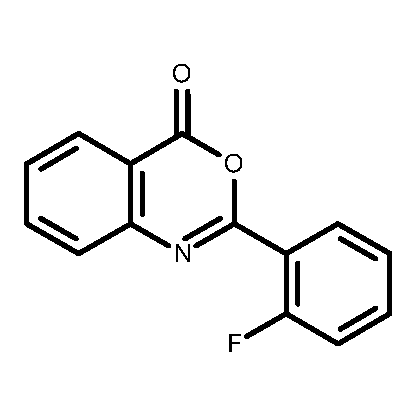
\includegraphics[width = 0.14\textwidth]{2DImages/SAMPL5_003.pdf} & 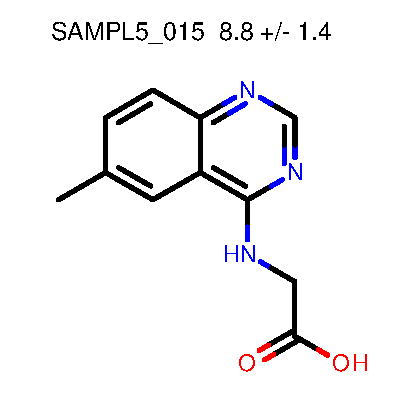
\includegraphics[width = 0.14\textwidth]{2DImages/SAMPL5_015.pdf} & 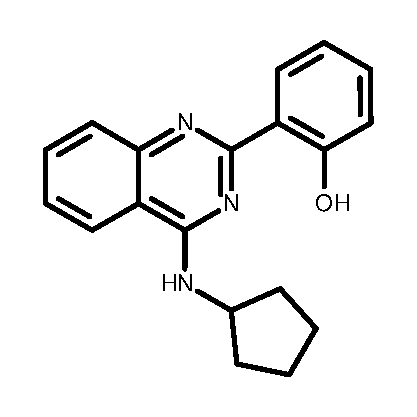
\includegraphics[width = 0.14\textwidth]{2DImages/SAMPL5_017.pdf} & 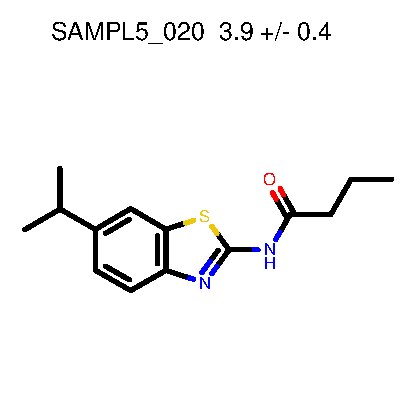
\includegraphics[width = 0.14\textwidth]{2DImages/SAMPL5_020.pdf} & 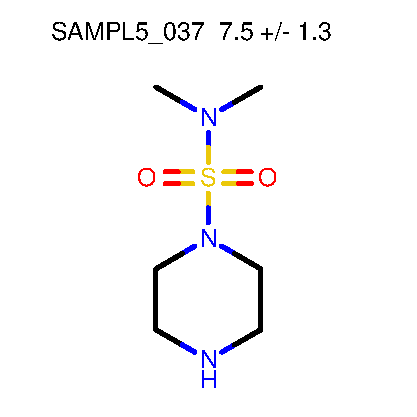
\includegraphics[width = 0.14\textwidth]{2DImages/SAMPL5_037.pdf} & 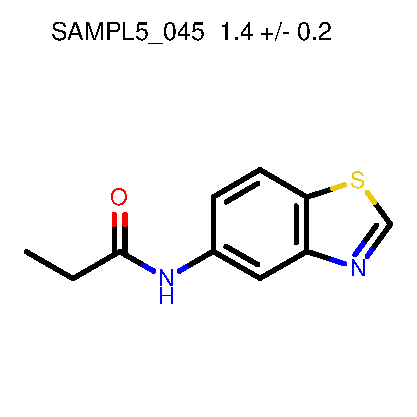
\includegraphics[width = 0.14\textwidth]{2DImages/SAMPL5_045.pdf} & 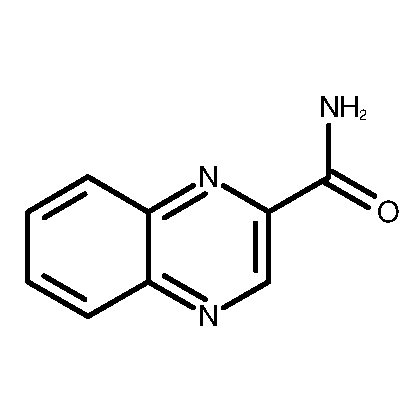
\includegraphics[width = 0.14\textwidth]{2DImages/SAMPL5_055.pdf} \\ 
{\scriptsize 058: $ 2.2 \pm 0.3 $ } & {\scriptsize 059: $ 1.8 \pm 0.2 $ } & {\scriptsize 061: $ 5.9 \pm 1.0 $ } & {\scriptsize 068: $ 2.7 \pm 0.3 $ } & {\scriptsize 070: $ 5.9 \pm 0.8 $ } & {\scriptsize 080: $ 2.6 \pm 0.2 $ } & \\ 
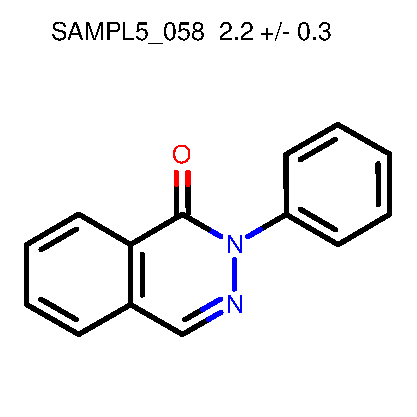
\includegraphics[width = 0.14\textwidth]{2DImages/SAMPL5_058.pdf} & 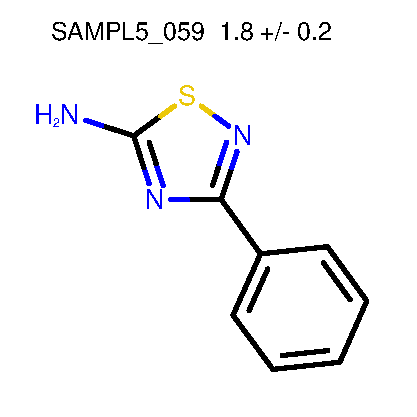
\includegraphics[width = 0.14\textwidth]{2DImages/SAMPL5_059.pdf} & 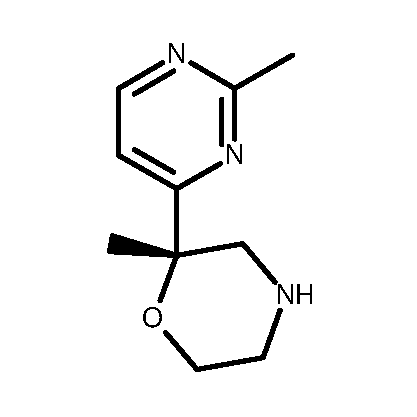
\includegraphics[width = 0.14\textwidth]{2DImages/SAMPL5_061.pdf} & 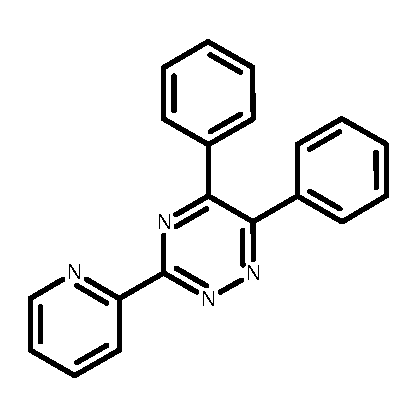
\includegraphics[width = 0.14\textwidth]{2DImages/SAMPL5_068.pdf} & 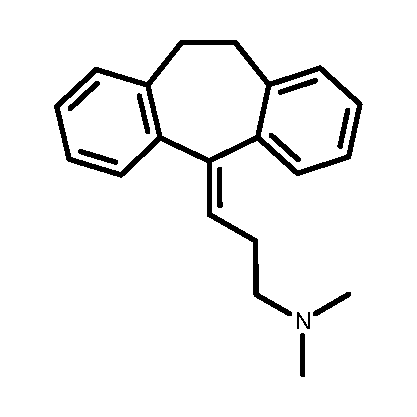
\includegraphics[width = 0.14\textwidth]{2DImages/SAMPL5_070.pdf} & 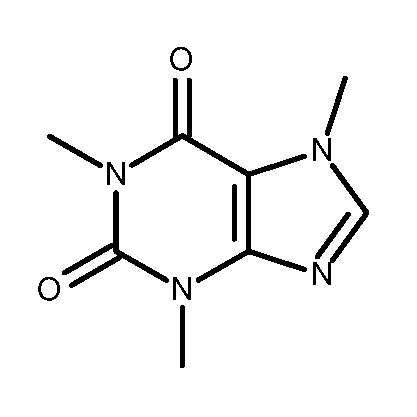
\includegraphics[width = 0.14\textwidth]{2DImages/SAMPL5_080.pdf} & \\ 
\hline 
\multicolumn{7}{|c|}{{\small\textbf{Batch 1}}}\\ 
{\scriptsize 004: $ 2.3 \pm 0.3 $ } & {\scriptsize 005: $ 2.6 \pm 0.3 $ } & {\scriptsize 007: $ 3.1 \pm 0.4 $ } & {\scriptsize 010: $ 7.8 \pm 1.6 $ } & {\scriptsize 011: $ 7.1 \pm 1.3 $ } & {\scriptsize 021: $ 2.2 \pm 0.2 $ } & {\scriptsize 026: $ 8.0 \pm 1.7 $ } \\ 
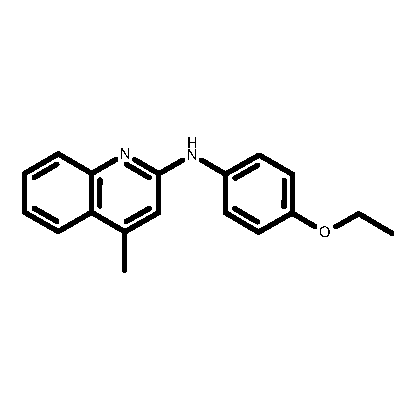
\includegraphics[width = 0.14\textwidth]{2DImages/SAMPL5_004.pdf} & 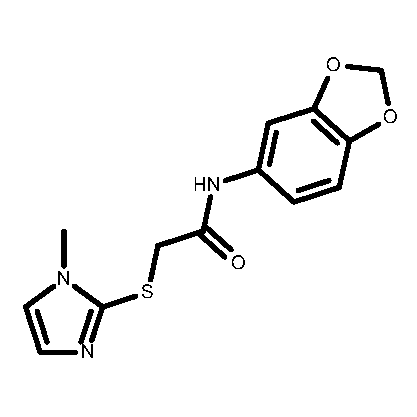
\includegraphics[width = 0.14\textwidth]{2DImages/SAMPL5_005.pdf} & 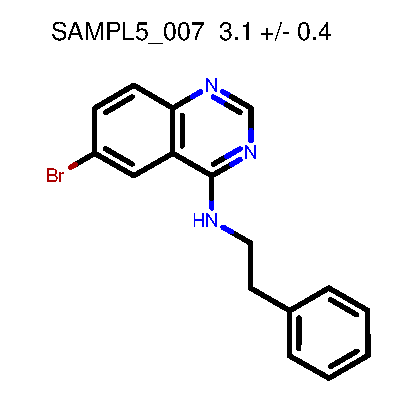
\includegraphics[width = 0.14\textwidth]{2DImages/SAMPL5_007.pdf} & 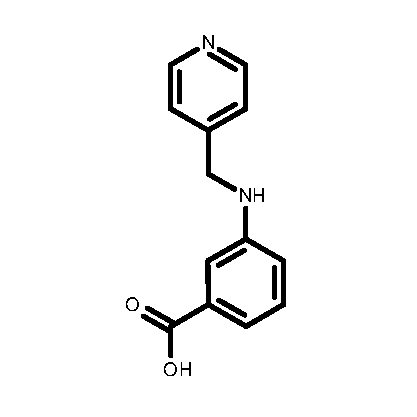
\includegraphics[width = 0.14\textwidth]{2DImages/SAMPL5_010.pdf} & 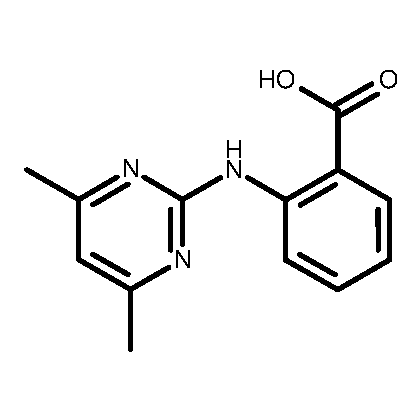
\includegraphics[width = 0.14\textwidth]{2DImages/SAMPL5_011.pdf} & 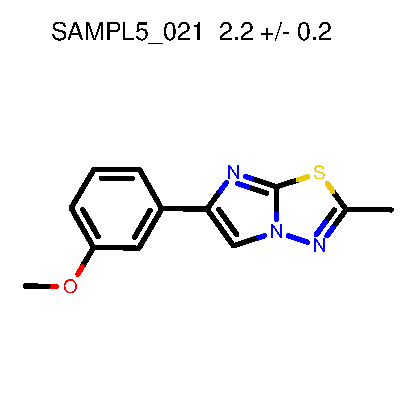
\includegraphics[width = 0.14\textwidth]{2DImages/SAMPL5_021.pdf} & 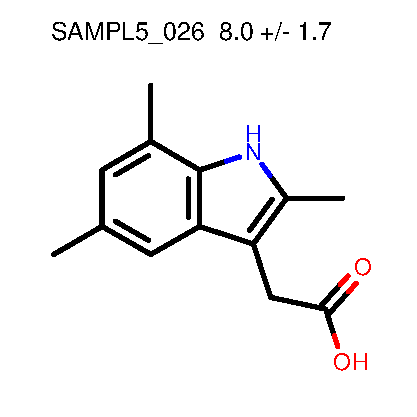
\includegraphics[width = 0.14\textwidth]{2DImages/SAMPL5_026.pdf} \\ 
{\scriptsize 027: $ 3.4 \pm 0.3 $ } & {\scriptsize 042: $ 3.2 \pm 0.4 $ } & {\scriptsize 044: $ 3.7 \pm 0.4 $ } & {\scriptsize 046: $ 2.7 \pm 0.4 $ } & {\scriptsize 047: $ 2.1 \pm 0.3 $ } & {\scriptsize 048: $ 2.7 \pm 0.3 $ } & {\scriptsize 056: $ 3.5 \pm 0.3 $ } \\ 
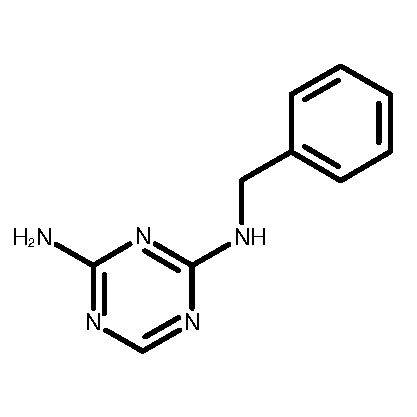
\includegraphics[width = 0.14\textwidth]{2DImages/SAMPL5_027.pdf} & 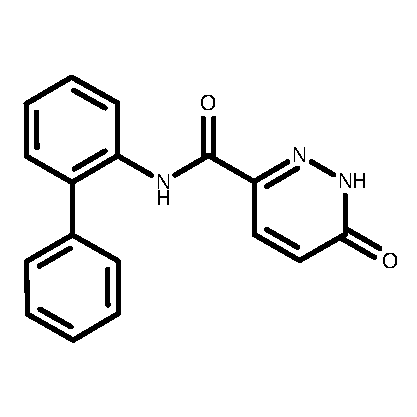
\includegraphics[width = 0.14\textwidth]{2DImages/SAMPL5_042.pdf} & 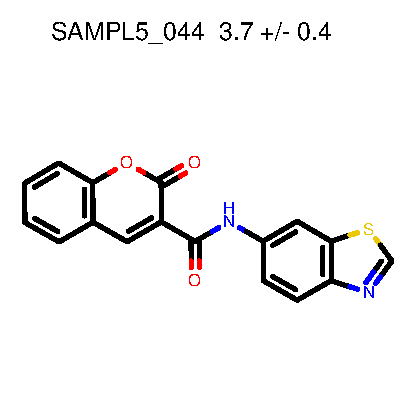
\includegraphics[width = 0.14\textwidth]{2DImages/SAMPL5_044.pdf} & 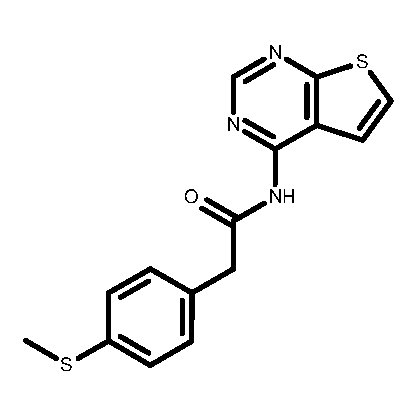
\includegraphics[width = 0.14\textwidth]{2DImages/SAMPL5_046.pdf} & 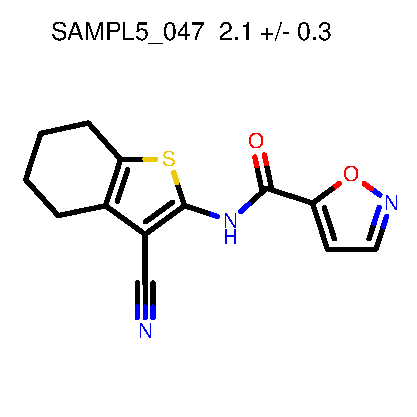
\includegraphics[width = 0.14\textwidth]{2DImages/SAMPL5_047.pdf} & 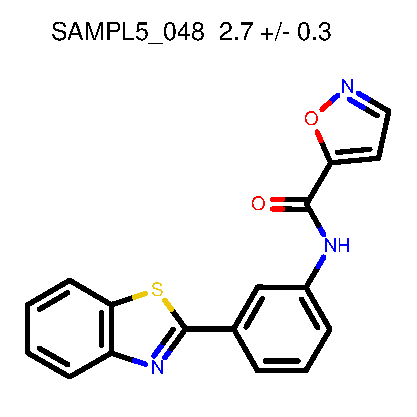
\includegraphics[width = 0.14\textwidth]{2DImages/SAMPL5_048.pdf} & 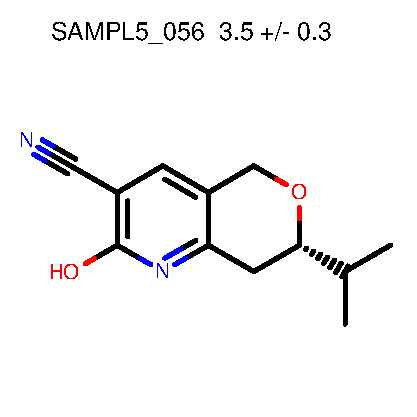
\includegraphics[width = 0.14\textwidth]{2DImages/SAMPL5_056.pdf} \\ 
{\scriptsize 060: $ 6.7 \pm 1.6 $ } & {\scriptsize 063: $ 6.7 \pm 1.0 $ } & {\scriptsize 071: $ 2.8 \pm 0.3 $ } & {\scriptsize 072: $ 4.9 \pm 0.7 $ } & {\scriptsize 081: $ 6.0 \pm 0.8 $ } & {\scriptsize 090: $ 2.8 \pm 0.3 $ } & \\ 
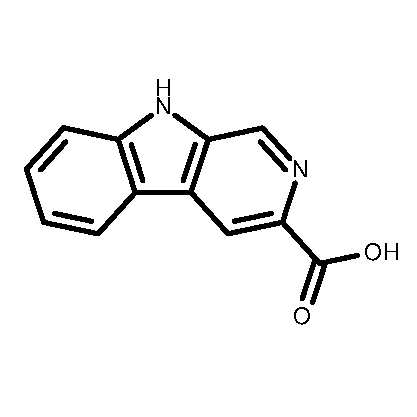
\includegraphics[width = 0.14\textwidth]{2DImages/SAMPL5_060.pdf} & 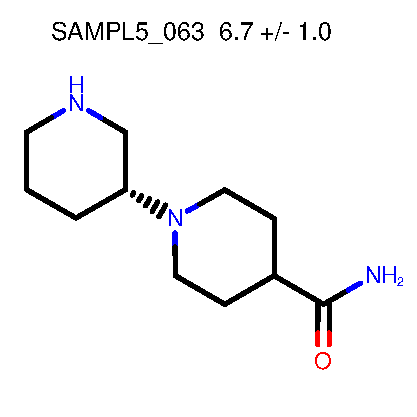
\includegraphics[width = 0.14\textwidth]{2DImages/SAMPL5_063.pdf} & 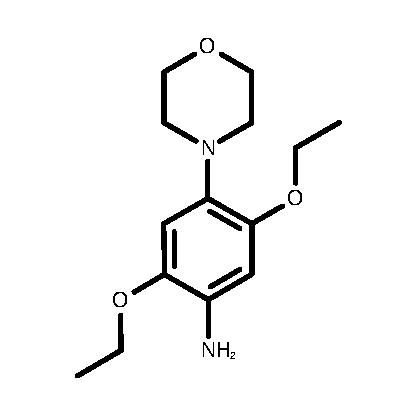
\includegraphics[width = 0.14\textwidth]{2DImages/SAMPL5_071.pdf} & 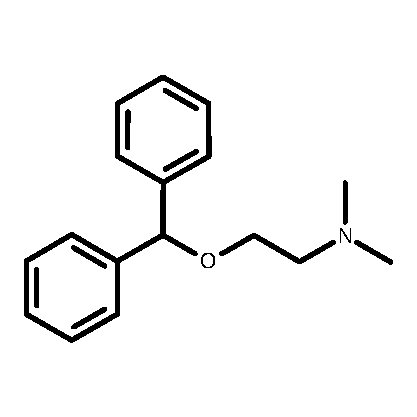
\includegraphics[width = 0.14\textwidth]{2DImages/SAMPL5_072.pdf} & 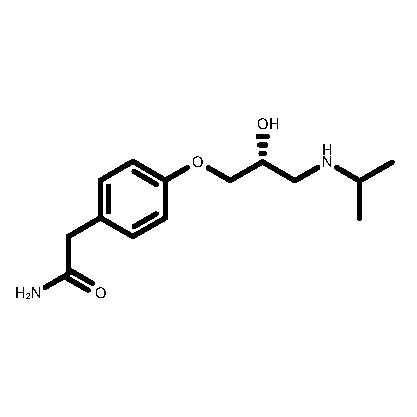
\includegraphics[width = 0.14\textwidth]{2DImages/SAMPL5_081.pdf} & 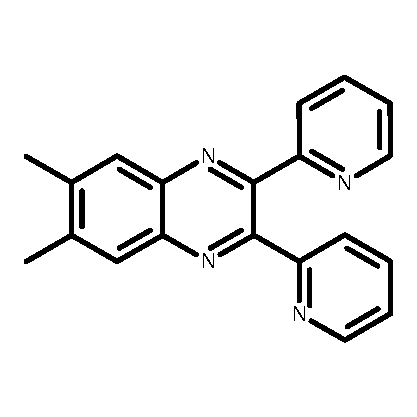
\includegraphics[width = 0.14\textwidth]{2DImages/SAMPL5_090.pdf} & \\ 
\hline 
\multicolumn{7}{|c|}{{\small\textbf{Batch 2}}}\\ 
{\scriptsize 002: $ 2.5 \pm 0.2 $ } & {\scriptsize 006: $ 2.7 \pm 0.4 $ } & {\scriptsize 013: $ 3.1 \pm 0.3 $ } & {\scriptsize 019: $ 3.1 \pm 0.4 $ } & {\scriptsize 024: $ 3.0 \pm 0.4 $ } & {\scriptsize 033: $ 3.0 \pm 0.3 $ } & {\scriptsize 049: $ 2.1 \pm 0.2 $ } \\ 
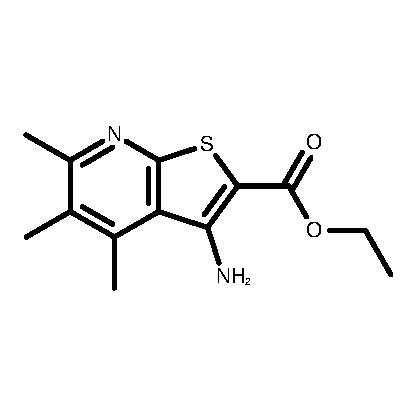
\includegraphics[width = 0.14\textwidth]{2DImages/SAMPL5_002.pdf} & 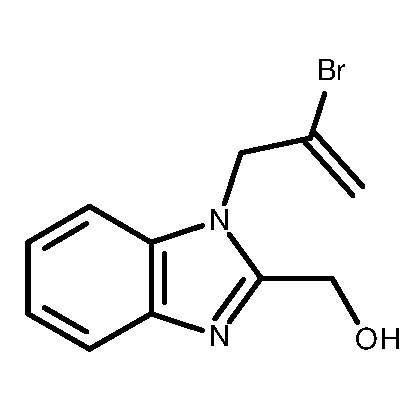
\includegraphics[width = 0.14\textwidth]{2DImages/SAMPL5_006.pdf} & 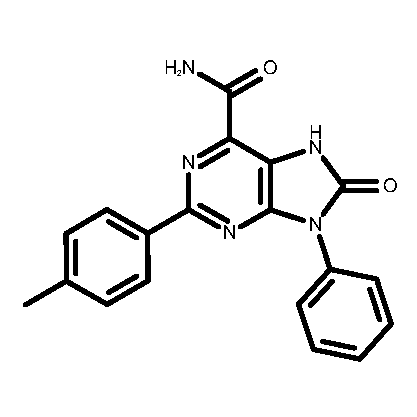
\includegraphics[width = 0.14\textwidth]{2DImages/SAMPL5_013.pdf} & 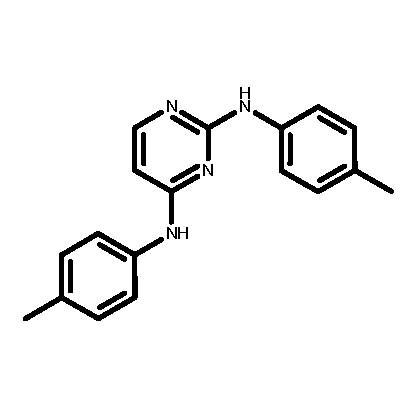
\includegraphics[width = 0.14\textwidth]{2DImages/SAMPL5_019.pdf} & 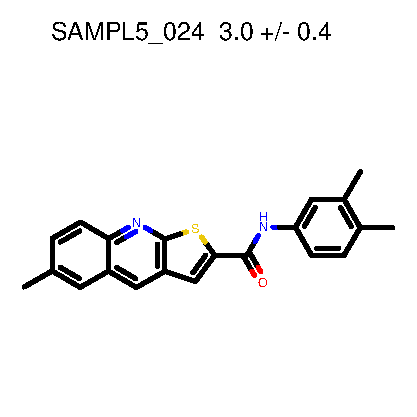
\includegraphics[width = 0.14\textwidth]{2DImages/SAMPL5_024.pdf} & 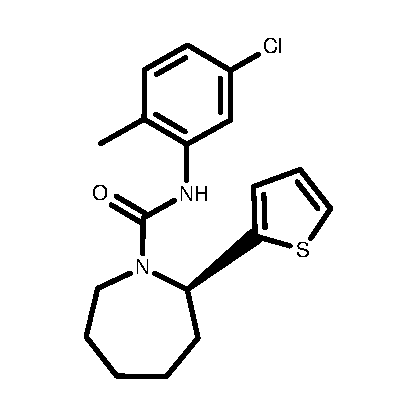
\includegraphics[width = 0.14\textwidth]{2DImages/SAMPL5_033.pdf} & 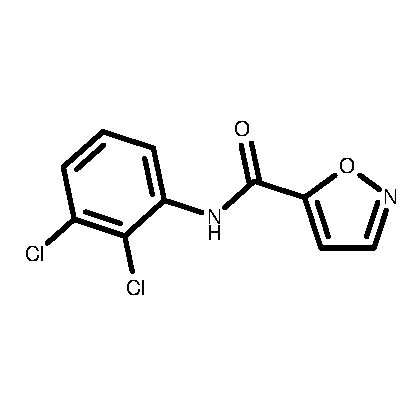
\includegraphics[width = 0.14\textwidth]{2DImages/SAMPL5_049.pdf} \\ 
{\scriptsize 050: $ 5.6 \pm 0.4 $ } & {\scriptsize 065: $ 5.3 \pm 0.5 $ } & {\scriptsize 067: $ 4.5 \pm 0.6 $ } & {\scriptsize 069: $ 3.9 \pm 0.5 $ } & {\scriptsize 074: $ 6.6 \pm 0.4 $ } & {\scriptsize 075: $ 4.8 \pm 0.6 $ } & {\scriptsize 082: $ 5.1 \pm 0.6 $ } \\ 
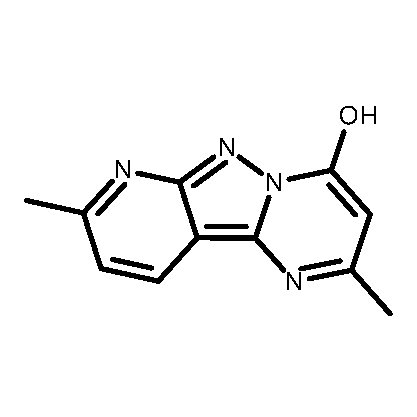
\includegraphics[width = 0.14\textwidth]{2DImages/SAMPL5_050.pdf} & 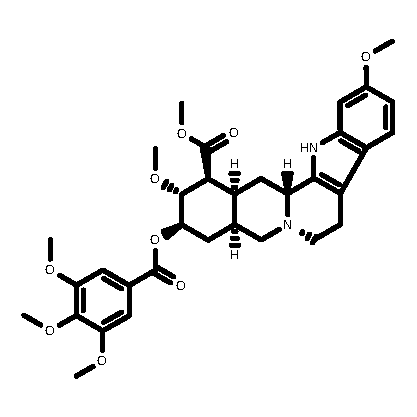
\includegraphics[width = 0.14\textwidth]{2DImages/SAMPL5_065.pdf} & 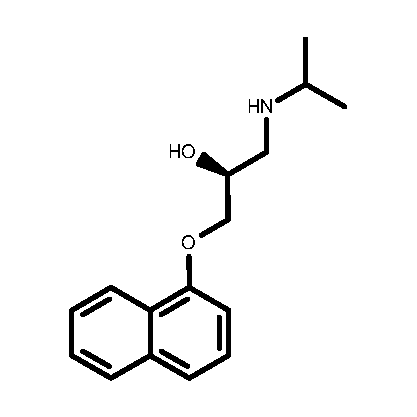
\includegraphics[width = 0.14\textwidth]{2DImages/SAMPL5_067.pdf} & 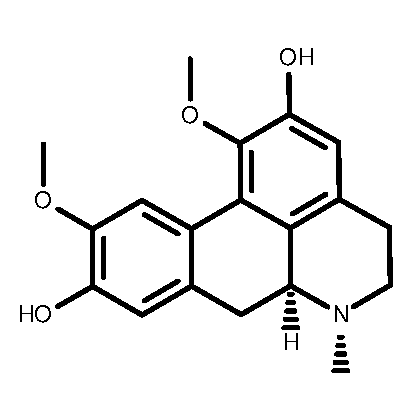
\includegraphics[width = 0.14\textwidth]{2DImages/SAMPL5_069.pdf} & 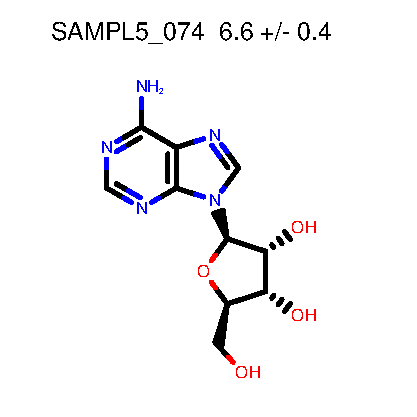
\includegraphics[width = 0.14\textwidth]{2DImages/SAMPL5_074.pdf} & 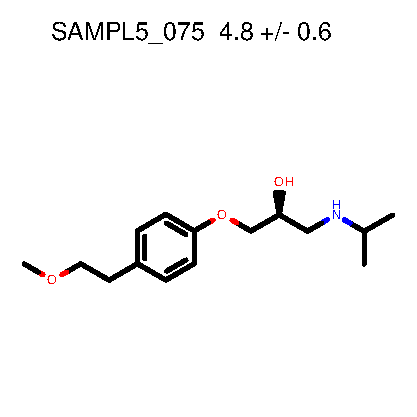
\includegraphics[width = 0.14\textwidth]{2DImages/SAMPL5_075.pdf} & 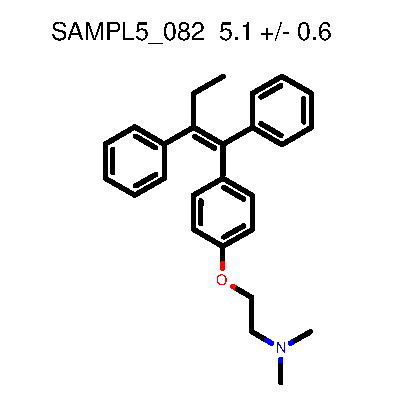
\includegraphics[width = 0.14\textwidth]{2DImages/SAMPL5_082.pdf} \\ 
{\scriptsize 083: $ 8.4 \pm 0.7 $ } & {\scriptsize 084: $ 3.6 \pm 0.5 $ } & {\scriptsize 085: $ 2.8 \pm 0.3 $ } & {\scriptsize 086: $ 4.5 \pm 0.6 $ } & {\scriptsize 088: $ 2.9 \pm 0.4 $ } & {\scriptsize 092: $ 3.9 \pm 0.4 $ } & \\ 
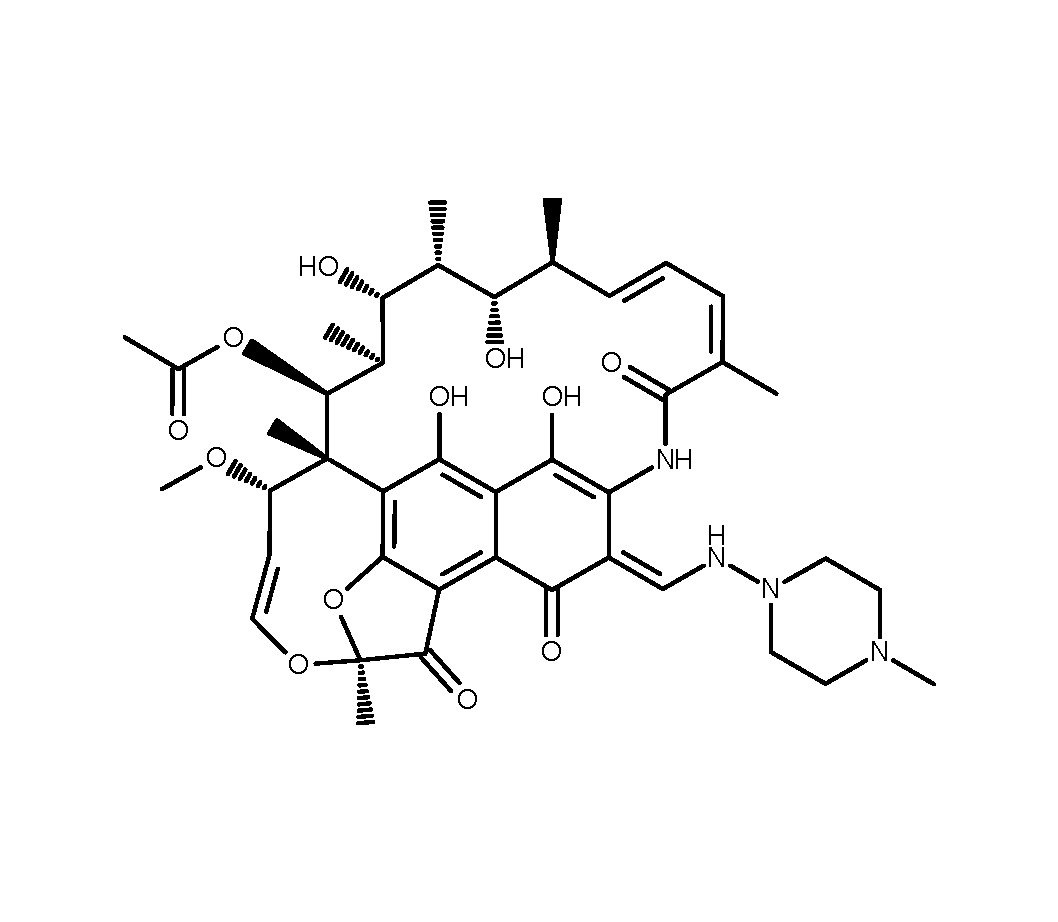
\includegraphics[width = 0.14\textwidth]{2DImages/SAMPL5_083.pdf} & 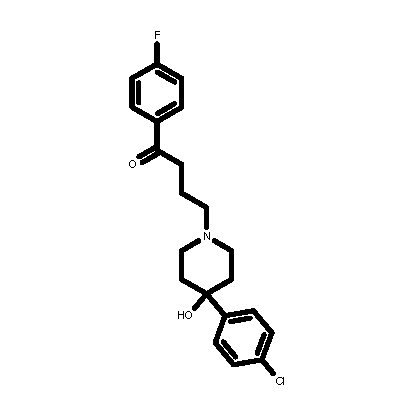
\includegraphics[width = 0.14\textwidth]{2DImages/SAMPL5_084.pdf} & 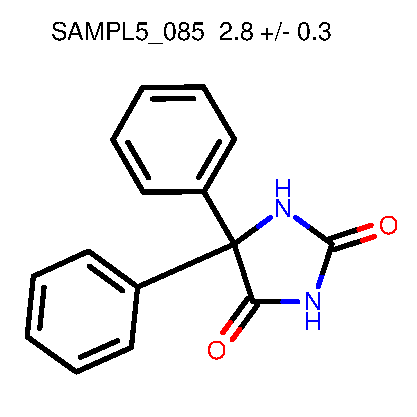
\includegraphics[width = 0.14\textwidth]{2DImages/SAMPL5_085.pdf} & \includegraphics[width = 0.14\textwidth]{2DImages/SAMPL5_086.pdf} & \includegraphics[width = 0.14\textwidth]{2DImages/SAMPL5_088.pdf} & \includegraphics[width = 0.14\textwidth]{2DImages/SAMPL5_092.pdf} & \\ 
\hline
\end{tabular}

\label{MoleculeTable}
\caption{A complete list of compounds used in the SAMPL5 challenge, sorted by batch. The average unsigned error (AUE), reported in log units as SAMPL5 ID: AUE, was calculated with all submitted predictions for that compound. The 2D images were generated using OpenEye OEDepict toolkit  \cite{openeye} using the provided SMILES strings.} 
\end{table}
% I rotated 083, it is a little more clear now

For the prediction of distribution coefficients in SAMPL5, a total of 53 molecules were considered. 
They were assigned an identifier in the form SAMPL5\_XXX and are pictured in table \ref{MoleculeTable}.  
The 53 molecules were divided into batches 0, 1, and 2 containing 13, 20, and 20 molecules respectively. 
We wanted each batch to have a similar dynamic range and for the molecules to increase in size across batches, so on average the smallest molecules are in batch 0 and the largest in batch 2. 
To ensure each batch had adequate dynamic range, the molecular weight and estimated octanol/water partition coefficient were computed for each compound. 
These partition coefficients were estimated with OpenEye's $\log P$ calculator. Molecules were then assigned to bins by estimated partition coefficient, and assigned to batches based on molecular weight. 
Specifically, the smallest molecules from each partition coefficient bin were added to batch 0, then batch 1, and the rest of the molecules comprise batch 2.

Participants could submit partial sets of predictions as long as they included full consecutive batches; that is, they could submit batch 0, batches 0 and 1, or batches 0, 1, and 2. 
The idea was that all participants should attempt predictions on the full set if at all possible, but grouping into batches would allow people with particularly demanding methods (such as polarizable force fields or methods requiring intensive quantum mechanics) to focus on smaller compounds and still be evaluated. 
Eight submissions from two participants included results for only batch 0, and an additional five submissions from two participants provided only batches 0 and 1.
Here we focus on the results for the complete set of molecules (batches 0, 1, and 2). 
Separate analysis for data subsets is available in the supporting information on Dash

Participants were asked to report a cyclohexane/water distribution coefficient for each molecule. 
As discussed above, distribution coefficients are the ratio of concentrations for all forms of the solute in the cyclohexane and aqueous layers, at a specified pH. 
In this case, experiments were done with the water layer consisting of a buffered aqueous solution at pH 7.4. 
We also required participants to provide two estimates for uncertainty, a statistical uncertainty for their computational method and a model uncertainty that estimates agreement with experiment.  
The statistical uncertainty was intended to be the variation expected over repeated calculations of the same value. 
The model uncertainty, on the other hand, was intended to provide an estimate of how well the calculated value will agree with experiment. 
For example, in a recent study we computed cyclohexane/water partition coefficients using alchemical solvation free energy calculations in GROMACS where the statistical uncertainties were around 0.05 log units,
but the root mean squared error was around 1.4 log units  \cite{Bannan:2016lp}, so an appropriate estimated model uncertainty would have been 1.4 log units. A careful analysis of expected error could even yield model uncertainties which would vary based on the anticipated difficulty or complexity of a compound. 
Our interest in model uncertainties is in part based on the realization that an important part of creating predictive models is the ability to know when they will be unreliable or fail. 
Thus, analysis of model uncertainties is an important part of evaluating any model. 

\section{Analysis of Submission Performance}
\label{analysisMethods}

As in past SAMPL challenges, we considered a variety of error metrics in analyzing all predictions submitted to SAMPL5. 
Each error metric was calculated for all submissions, by batch, and distributed to challenge participants before the workshop. % by batch?
Here we will focus primarily on six error metrics: the root-mean-squared error (RMSE), average unsigned error (AUE), average signed error (ASE), Pearson's R (R), Kendall's tau (tau), and the `error slope' explained in depth below. 
We also calculated the maximum absolute error and the percent of predictions with the correct sign, but these are not included in the analysis here.
However, these metrics were provided to challenge participants and are available in the supporting information on Dash.
The uncertainty in each metric was calculated as the standard deviation over 1000 bootstrap trials, where each trial consists of creating a `new' dataset by sampling pairs of (predicted, calculated) values from the original set, with replacement. 
As described previously, this bootstrapping technique also included variation in the experimental values based on their reported uncertainties \cite{Mobley:2014gu}.

As discussed above, an important factor influencing the utility of a predictive tool is the ability of the tool to not only provide predictions but to predict the accuracy of those predictions -- that is, how well the calculated values are likely to agree with experiment -- not just its statistical error.  
To assess this, as in SAMPL4  \cite{Mobley:2014gu}, a quantile-quantile plot (QQ Plot) was created for each prediction set  \cite{Wilk:1968cm}. 
QQ Plots compare the fraction of a normal distribution within a specified number of standard deviations to the distribution of errors (calculated minus experiment) that are within that number of model uncertainties.
For example, consider the number of predictions within one standard deviation of the expected value; if the samples are drawn from a normal distribution, then $~0.68$ of the values ought to fall within one standard deviation, so the value on the x-axis is $0.68$. The value on the y-axis will represent the fraction of predictions that are within one model uncertainty of the experimental value.  If the model uncertainty is accurate, then this also ought to correspond to a value of $0.68$.
A linear regression analysis helps summarize these results.
The `error slope' is the slope of the line comparing the fraction of predictions within a specified range of experiment to the expected fraction from a normal distribution.
An error slope of greater than one indicates that the calculated values are within uncertainty of experiment more often than expected, or in other words the model uncertainty was overestimated. 
In contrast, an error slope less than one suggests the model uncertainty was underestimated. 

We also attempted to identify any individual molecules where most of the methods failed to accurately estimate the distribution coefficient. 
To accomplish this, we analyzed all predictions on a molecule-by-molecule basis via our usual set of error metrics.  
Here we will primarily focus on just average unsigned error for molecules, but all other error metrics were provided to participants and are available in supporting information on Dash.

\section{Reference calculations} 
\label{methods:1}

We calculated distribution coefficients through a few different methods as a reference. 
K.H.B., a graduate student in the Mobley group, performed a set of blind calculations estimating the $\log D$ as a partition coefficient between cyclohexane and water calculated from solvation free energies.
In addition, C.C.B. and D.L.M. performed post-challenge analysis of protonation and tautomeric states and used this to convert our calculated partition coefficients to distribution coefficients.
We considered a null hypothesis where all molecules are assumed to distribute equally between cyclohexane and water.
Many fast structure-based tools for octanol/water partition coefficients exist, and we used one of those to estimate partition coefficients, both with no correction for the fact that we are interested in cyclohexane, and with a small adjustment for this as discussed below. 

\subsection{Calculating partition coefficients from solvation free energies}
\label{methods:2}
We decided to estimate distribution coefficients via a $\log P$ calculation, by assuming only a single neutral tautomer of each solute, then calculating $\log P$ from a difference in solvation free energies. 
Before the challenge, each molecule was taken directly from the provided SMILES string.
As demonstrated in the literature,  \cite{Essex:1992bd,Best:1999ix,JohnEEksterowicz:1997cj,Jorgensen:1989ga,Jorgensen:1990ha,Garrido:2009hz,Garrido:2011es,Garrido:2012gc,Yang:2013io,Michel:2007gw,Genheden:2016jj}
partition coefficients are directly proportional to the difference between the solvation free energy for the solute into each solvent. 
We use previously established and automated protocols  \cite{Bannan:2016lp} 
to calculate the solvation free energy of each molecule into water and cyclohexane. 
Then the calculated partition coefficient was reported as an estimate for $\log D$. 

To calculate solvation free energies, we used automated tools created by the Mobley lab.
Molecular dynamics simulations were performed in GROMACS   \cite{Berendsen:1995gro,Hess:2008db,Lindahl:2001gro3,vanderSpoel:2005hz,Pronk:2013ef,Pall:2014gb,Abraham:2015gj}
with the General AMBER Force Field (GAFF)  \cite{Wang:2004dev} with AM1-BCC charges  \cite{Jakalian:2000ki,Jakalian:2002bd}.
The TIP3P water model  \cite{Jorgensen:1983fl} was used for the aqueous phase. 
Topology and coordinate files for the solvated boxes with 1 solute molecule and 500 cyclohexane or 1000 water molecules were built using our Solvation Toolkit  \cite{Bannan:2016lp}.
These files were then converted to AMBER, DESMOND, and LAMMPS formats and provided to SAMPL5 participants as reference calculations.
The Solvation Toolkit takes advantage of many open source Python modules and is available at https://github.com/MobleyLab/SolvationToolkit.
It converts SMILES strings or IUPAC names of any mixture of small organic compounds to parameterized molecules and builds topology and coordinate files for a variety of simulation packages. 
All molecular dynamics parameters are identical to previous studies  \cite{Liu:2016kb,Klimovich:2010jm,Bannan:2016lp}.
The molecule is taken from the solvated box to a non-interacting gas phase in 20 lambda values. 
Solvation free energies are calculated with Alchemical Analysis tool  \cite{Klimovich:2015er} using the multi-state Bennett acceptance ratio to extract the free energy difference between the beginning and end state. 
The partition coefficient was calculated as the difference between the cyclohexane solvation free energy and the hydration free energy.
The statistical uncertainty was reported as the propagated uncertainty from the solvation free energy calculations. 
The model uncertainty was estimated to be the same for all molecules and reported as the root-mean-squared error from a recent study on calculating cyclohexane/water partition coefficient, specifically 1.4 log units  \cite{Bannan:2016lp}.
These reference calculations were assigned submission ID 39 and included in the error analysis performed on all submissions.

\paragraph{Simulation box size does not affect the calculated solvation free energy.} 
Hydration free energies were previously shown to be independent of box size for box edges ranging from 2 to 9 nanometers, within calculated uncertainties  \cite{Parameswaran:2014kq}; however, here, because cyclohexane is much less polar, we had some concern that finite size effects could still be significant. 
To explore this, we performed some tests in which we varied the simulation box size.
Because more polar solutes are more likely to have substantial long range interactions, we calculated the dipole moment of each SAMPL5 molecule using the position and charges on atoms in the mol2 files. 
SAMPL5\_024 had the largest dipole moment so it was used as the solute for the box size investigation. 
The solvation free energy calculations were set up as described above, changing the number of cyclohexane molecules from 100 to 500.  
Our calculations above are performed with lattice-sum (PME) treatment of coulomb interactions.
It was the primary focus of this check and we included duplicate calculations for the smaller box sizes where the initial coordinate file was the same, but new velocities were generated for the equilibrium phases. 
We also repeated the solvation free energy calculations with reaction field coulomb interactions assigning the dielectric coefficient for cyclohexane, 2.0243  \cite{crc}.
\begin{figure} 
\includegraphics{boxSize.eps}
\caption{Calculated solvation free energy for SAMPL5\_024 is independent of box size for PME and reaction field coulomb interactions. Points are connected to help distinguish between the two data sets}
\label{boxSizes}  
\end{figure}
For both types of simulation, the calculated solvation free energy fluctuated around an average of $19.1$ kcal/mol with no trend that would suggest solvation free energy depends on box size (figure \ref{boxSizes}).
There are many other explanations for fluctuations in calculated solvation free energies, including sampling, that might account for the $0.48$ kcal/mol range in the PME simulations. 
Ultimately, we find that box edge lengths from 2.64 to 4.54 nm have no significant affect on the calculated solvation free energies. 
This suggests that in the future, smaller box sizes could be used for computational efficiency. 
The input, results, molecular dynamics parameter and coordinate files, and tables of solvation free energies are available in the supporting information on Dash.
\subsection{Consideration of tautomers after SAMPL5}
\label{methods:3}

To help understand how the results from our partition coefficient calculations could have been improved, we considered corrections for changes in the solutes' protonation or tautomeric states.  
Distribution coefficients differ from partition coefficients in that they include all forms of the solute in both solvents. 
A common way to convert between experimentally measured distribution coefficients and partition coefficients is with pKa values for the solute  \cite{Sangster:1989tp}.
This is a simple correction using the Henderson-Hasselbalch 
equation:
\begin{equation}
pH = pK_a + \log \frac{[X]}{[HX]}
\label{HH}
\end{equation}
to relate the concentration of neutral species to the charged species at a given pH. 
This correction assumes the solute only has one other relevant protonation state and changes for acidic and basic molecules. 
Zwitterions and other neutral tautomers are not taken into account. 
The equation used to calculate a distribution coefficient ($\log D$) from a partition coefficient ($\log P$) for a basic solute (or $X$ in equation \ref{HH}) is below  
\begin{equation}
\log D = \log P - log(1+10^{pK_a-pH})
\label{basic}
\end{equation}
Alternatively for an acidic solute (or $HX$ in equation \ref{HH}) we would instead use:
\begin{equation}
\log D = \log P - log(1+10^{pH-pK_a})
\label{acidic}
\end{equation}
We use Schr\"{o}dinger's Epik tool  \cite{epik,Shelley:2007ku,Greenwood:2010hh} to estimate pKa values for each molecule according to experimental conditions. 
We then estimated $\log D$ using the equations above, accounting for just one change in protonation state, meaning each solute was taken to be either acidic or basic.
For acidic solutes, the smallest acidic pKa was used with equation \ref{acidic}, oppositely for basic solutes the largest basic pKa was used with equation \ref{basic} to estimate $\log D$ from $\log P$. 

Using pKa values only accounts for one change in protonation, whereas a correct distribution coefficient should include all relevant tautomers and protonation states of the molecule in both solvents. 
To account for all other tautomer states, we used Schr\"{o}dinger's LigPrep  \cite{ligprep} to enumerate tautomers for each molecule in the aqueous solution. 
The results of the enumeration can include an energetic ``state penalty'' calculated with Epik which relates the population of that tautomer to all others. 
This state penalty can be converted into log units and used as a correction term to convert $\log P$ to $\log D$:
\begin{equation}
\log D = \log P + \frac{-E_{state\ penalty}}{k_BT \ln (10)}
\label{statepenalty}
\end{equation}
where $k_B$ is Boltzmann constant and T is temperature. 
LigPrep can only perform the tautomer enumeration with water or DMSO as a solvent, so we were unable to predict tautomers in cyclohexane. 
Therefore both of these corrections account for the protonation or tautomer states only in the aqueous layer and assume the tautomer remains fixed in cyclohexane as the one used in the initial simulation. In the results section below, the corrections performed with $pK_a$ and the corrections made with the the calculated state penalty are referred to $\log D_{pK_a}$ and $\log D_{state\ penalty}$ respectively. 

\subsection{Estimating distribution coefficients with a fast, structural based partition coefficient calculator}
\label{methods:4}
Many structure-based tools exist for octanol/water partition coefficients; they are very fast and generally accurate. 
However, these tools are all trained on empirical data, meaning they are limited by the training data. 
We chose the OpenEye tool OEXlogP  \cite{RenxiaoWang:1997fa,Wang:2000kk} as an example of such a tool. 
Two post-prediction sets were prepared with the OEXlogP tool.
First, the predicted octanol/water partition coefficient was considered an estimate for cyclohexane/water distribution coefficient.
In the second set, we used a linear regression to correct for the bias between the calculated XlogP values and a set of experimental cyclohexane/water partition coefficients  \cite{Leo:1971wu}.
For the rest of this paper we will refer to the octanol/water partition coefficient set as $XlogP_{oct}$ and the bias-corrected set as $XlogP_{corr}$. 

\subsection{Exploring the possibility of mixing solvents}
Because no two solvents are perfectly immiscible, we wanted to explore the effect that a small amount of water present in cyclohexane would have on computed $\log D$ values for one of the more polar solutes. 
The experimental concentration of water in cyclohexane is 0.00047 mole fraction \cite{Black:1948bs}. 
The presence of water in the cyclohexane phase has a possibility of affecting the transfer free energy, especially for solutes with many polar functional groups. 
Also, it has been suggested that particularly polar compounds can pull water with them from the aqueous layer into the organic solvent \cite{Leo:1971wu}; while this is a kinetic argument and should not apply to equilibrium thermodynamic properties like $\log D$, the point is well taken --- some solutes have a particularly high affinity for water and may actually impact the amount of water present in cyclohexane when the solute is present at finite concentration.
Thus, to investigate this, we took one of the most polar compounds -- one for which we had particularly large errors relative to experiment -- SAMPL5\_074, and performed two additional sets of free energy calculations in cyclohexane. 
Both sets of simulations had the single solute in 150 cyclohexane molecules, but varied in water content -- the first with seven water molecules present in cyclohexane, and the second with only a single water molecule.  
The input files for these simulations were also created with Solvation Toolkit as described above and the same simulation protocol was followed. 
These simulations were conducted after the SAMPL submission deadline in order to help us understand the role of water in such cases.

The experiments were not done on completely pure water and cyclohexane -- particularly, experimental distribution coefficients were measured with small amounts of dimethyl sulfoxide (DMSO) and acetonitrile present in solution. 
Therefore, we investigated the how acetonitrile and DMSO would distribute in simulations. 
The experimental concentrations reported for each solvent are approximately 50\%, 50\%, 1\%, and 0.4\% by volume for cyclohexane, water, DMSO, and acetonitrile respectively  \cite{Rustenburg:sampl5}.
To explore how the DMSO and acetonitrile distribute between cyclohexane and water we performed a single simulation with 130 cyclohexane, 780 water, four DMSO, and two acetonitrile molecules mirroring those concentrations. 
Input topology and coordinate files were created with Solvation Toolkit. 
The system was minimized and equilibrated following our reference calculation procedure and then a 5 ns constant pressure and temperature production simulation was run. 
The trajectory from this simulation was visualized with VMD  \cite{VMD} and a movie is available in the supplementary information. 


\section{Results and Discussion}
\label{results:1}
A broad range of methods were used for the 76 submissions predicting cyclohexane/water distribution coefficients for the SAMPL5 challenge. 
Many of these predictions used alchemical molecular dynamics simulations to estimate the solvation free energy in explicit solvent using several classes of force fields, including fixed-charge all-atom force fields \cite{Paranahewage:sampl5,Iorga:sampl5,Bosisio:sampl5,Pickard:sampl5,Konig:sampl5},
all-atom/coarse-grained hybrid force fields \cite{Genheden:sampl5}, 
and polarizable force fields \cite{Kamath:sampl5}. 
One participant used Semi-Explicit Assembly, a type of implicit solvent solvation free energy method applied to one or more chosen solute conformations \cite{Brini:sampl5}. 
A variety of quantum mechanics (QM) methods were also used including QM/molecular mechanics (QM/MM) with explicit solvent \cite{Pickard:sampl5,Konig:sampl5}, 
QM with non-Boltzmann Bennett free energy calculations \cite{Pickard:sampl5,Konig:sampl5}, 
and QM energy calculations with a single optimized molecular geometry \cite{Pickard:sampl5,Jones:sampl5}. 
Two participants used variations on the reference interaction-site model (RISM), an integral equation approach, to predict solvation free energies \cite{Tielker:sampl5,Luchko:sampl5}. 
One participant used QM calculations to derive parameters to tune an empirical model for activity coefficients and used these to estimate distribution coefficients \cite{Paluch:sampl5}.
A few submissions used empirically trained methods for calculating solvation free energies \cite{Park:sampl5,Santos-Martins:sampl5}. 
A particularly successful submission, which will be discussed again below, employed the Conductor-Like-Screening Model for Real Solvents (COSMO-RS)  \cite{Klamt:sampl5}. 

SAMPL5 is the first SAMPL challenge to include distribution coefficients, but we can estimate how well we expect submissions to do based on past SAMPL challenges which included hydration free energies. 
Distribution coefficients can be related to transfer free energy between solvents, which allows us to estimate an expected performance from root-mean-squared error (RMSE) in past hydration free energy calculations. 
In SAMPL4  \cite{Mobley:2014gu}, the average RMSE for the best half of submissions was about 1.5 kcal/mol which would correspond to a 1.54 log unit error in a distribution coefficient if both solvation free energies have comparable errors. 
Here, only five submissions had an RMSE less than 2.5 log units in SAMPL5. 
There are many reasons for this perceived change in accuracy, such as a more complex set of molecules, the use of cyclohexane as a solvent, and the complexity of estimating tautomer populations, discussed in depth below. 
Since this is the first challenge on predicting distribution coefficients, it is likely that participants had not yet developed good protocols to deal with many of these challenges, meaning that somewhat less accuracy ought to be expected.
It took several challenges focused on hydration \cite{Mobley:2014gu,Geballe:2012fc,Geballe:2010jr,Klimovich:2010jm,Mobley:2009iu,Mobley:2012jwa,Nicholls:2008cx}  before a range of methods could achieve the success noted in SAMPL4.
 
\begin{table}
\scriptsize
\footnotesize
\begin{tabular}{l l l l l l l}
\hline
ID & Ave. err. & RMS & AUE & tau & R & Err. slope \\ 
\hline
01\textsuperscript{1} & $2.3 \pm 0.8$ & $5.1 \pm 0.5$ & $4.3 \pm 0.5$ & $0.13 \pm 0.12$ & $0.20 \pm 0.17$ & $0.44 \pm 0.09$ \\ 
02 & $-0.5 \pm 0.3$ & $2.3 \pm 0.3$ & $1.7 \pm 0.2$ & $0.48 \pm 0.07$ & $0.63 \pm 0.07$ & $0.69 \pm 0.07$ \\ 
03\textsuperscript{1} & $-7.6 \pm 3.5$ & $21.3 \pm 2.6$ & $15.9 \pm 2.5$ & $0.52 \pm 0.10$ & $0.59 \pm 0.12$ & $-0.00 \pm 0.00$ \\ 
04\textsuperscript{0} & $1.6 \pm 0.5$ & $2.5 \pm 0.6$ & $1.9 \pm 0.4$ & $0.77 \pm 0.12$ & $0.87 \pm 0.05$ & $0.77 \pm 0.12$ \\ 
05 & $-8.2 \pm 0.4$ & $8.7 \pm 0.5$ & $8.2 \pm 0.4$ & $0.29 \pm 0.09$ & $0.39 \pm 0.11$ & $0.21 \pm 0.03$ \\ 
06 & $1.8 \pm 0.5$ & $4.0 \pm 0.3$ & $3.4 \pm 0.3$ & $0.46 \pm 0.09$ & $0.61 \pm 0.10$ & $0.58 \pm 0.07$ \\ 
07 & $0.5 \pm 0.4$ & $3.3 \pm 0.4$ & $2.5 \pm 0.3$ & $0.34 \pm 0.08$ & $0.51 \pm 0.11$ & $0.33 \pm 0.07$ \\ 
08 & $-1.7 \pm 0.4$ & $3.5 \pm 0.5$ & $2.5 \pm 0.3$ & $0.58 \pm 0.06$ & $0.70 \pm 0.06$ & $0.60 \pm 0.08$ \\ 
09 & $6.5 \pm 0.6$ & $7.8 \pm 0.6$ & $6.5 \pm 0.6$ & $-0.29 \pm 0.08$ & $-0.40 \pm 0.10$ & $0.35 \pm 0.07$ \\ 
10 & $0.3 \pm 0.4$ & $3.1 \pm 0.3$ & $2.6 \pm 0.3$ & $0.51 \pm 0.07$ & $0.69 \pm 0.07$ & $0.79 \pm 0.07$ \\ 
11 & $-4.4 \pm 1.8$ & $13.3 \pm 2.6$ & $6.9 \pm 1.6$ & $0.45 \pm 0.09$ & $0.53 \pm 0.09$ & $0.39 \pm 0.08$ \\ 
12 & $-5.5 \pm 2.5$ & $19.4 \pm 1.8$ & $15.0 \pm 1.6$ & $0.37 \pm 0.09$ & $0.39 \pm 0.12$ & $-0.00 \pm 0.00$ \\ 
13\textsuperscript{0} & $-11.1 \pm 5.0$ & $21.0 \pm 4.9$ & $12.2 \pm 4.8$ & $0.56 \pm 0.16$ & $0.43 \pm 0.22$ & $0.59 \pm 0.17$ \\ 
14 & $-0.7 \pm 0.3$ & $2.7 \pm 0.4$ & $2.0 \pm 0.3$ & $0.57 \pm 0.06$ & $0.72 \pm 0.06$ & $0.66 \pm 0.08$ \\ 
15 & $-1.4 \pm 0.4$ & $3.3 \pm 0.5$ & $2.3 \pm 0.3$ & $0.57 \pm 0.07$ & $0.70 \pm 0.06$ & $0.61 \pm 0.07$ \\ 
16 & $0.5 \pm 0.3$ & $2.1 \pm 0.2$ & $1.7 \pm 0.2$ & $0.73 \pm 0.04$ & $0.84 \pm 0.04$ & $0.46 \pm 0.08$ \\ 
17 & $-4.2 \pm 0.4$ & $5.0 \pm 0.4$ & $4.2 \pm 0.4$ & $0.36 \pm 0.08$ & $0.51 \pm 0.10$ & $0.50 \pm 0.07$ \\ 
18 & $-0.8 \pm 0.4$ & $2.7 \pm 0.4$ & $2.0 \pm 0.3$ & $0.47 \pm 0.07$ & $0.60 \pm 0.08$ & $0.62 \pm 0.08$ \\ 
19 & $1.5 \pm 0.3$ & $2.7 \pm 0.2$ & $2.3 \pm 0.2$ & $0.54 \pm 0.07$ & $0.75 \pm 0.07$ & $0.83 \pm 0.06$ \\ 
20 & $-2.3 \pm 0.4$ & $3.6 \pm 0.5$ & $2.7 \pm 0.3$ & $0.55 \pm 0.07$ & $0.70 \pm 0.06$ & $0.48 \pm 0.08$ \\ 
21 & $-1.2 \pm 0.5$ & $3.4 \pm 0.7$ & $2.4 \pm 0.3$ & $0.44 \pm 0.08$ & $0.45 \pm 0.16$ & $0.58 \pm 0.08$ \\ 
22 & $1.6 \pm 0.5$ & $3.9 \pm 0.3$ & $3.1 \pm 0.3$ & $0.29 \pm 0.09$ & $0.48 \pm 0.11$ & $0.68 \pm 0.08$ \\ 
23 & $1.9 \pm 0.5$ & $4.0 \pm 0.4$ & $3.0 \pm 0.4$ & $0.42 \pm 0.07$ & $0.58 \pm 0.08$ & $0.78 \pm 0.08$ \\ 
24\textsuperscript{0} & $2.3 \pm 0.7$ & $3.3 \pm 0.8$ & $2.5 \pm 0.6$ & $0.77 \pm 0.13$ & $0.88 \pm 0.05$ & $0.67 \pm 0.15$ \\ 
25 & $0.0 \pm 0.5$ & $3.6 \pm 0.3$ & $2.9 \pm 0.3$ & $0.53 \pm 0.07$ & $0.70 \pm 0.07$ & $0.71 \pm 0.07$ \\ 
26 & $2.3 \pm 0.7$ & $5.6 \pm 0.4$ & $4.6 \pm 0.4$ & $0.25 \pm 0.08$ & $0.37 \pm 0.11$ & $0.46 \pm 0.07$ \\ 
27 & $-0.2 \pm 0.4$ & $2.6 \pm 0.4$ & $1.8 \pm 0.2$ & $0.49 \pm 0.07$ & $0.61 \pm 0.08$ & $0.66 \pm 0.08$ \\ 
28 & $-2.3 \pm 0.4$ & $3.6 \pm 0.4$ & $2.7 \pm 0.3$ & $0.54 \pm 0.07$ & $0.69 \pm 0.06$ & $0.47 \pm 0.07$ \\ 
29 & $-6.7 \pm 0.4$ & $7.2 \pm 0.4$ & $6.7 \pm 0.4$ & $0.33 \pm 0.08$ & $0.45 \pm 0.11$ & $0.28 \pm 0.04$ \\ 
30 & $2.5 \pm 0.5$ & $4.3 \pm 0.3$ & $3.7 \pm 0.3$ & $0.39 \pm 0.10$ & $0.52 \pm 0.11$ & $0.53 \pm 0.07$ \\ 
31 & $-1.0 \pm 0.3$ & $2.7 \pm 0.3$ & $2.0 \pm 0.3$ & $0.56 \pm 0.07$ & $0.72 \pm 0.06$ & $0.63 \pm 0.08$ \\ 
32 & $2.5 \pm 0.4$ & $3.5 \pm 0.3$ & $3.1 \pm 0.2$ & $0.47 \pm 0.06$ & $0.64 \pm 0.07$ & $0.25 \pm 0.06$ \\ 
33 & $-0.1 \pm 0.5$ & $3.4 \pm 0.3$ & $2.8 \pm 0.3$ & $0.53 \pm 0.08$ & $0.71 \pm 0.08$ & $0.73 \pm 0.07$ \\ 
34 & $-1.3 \pm 0.4$ & $3.0 \pm 0.4$ & $2.2 \pm 0.3$ & $0.56 \pm 0.06$ & $0.69 \pm 0.07$ & $0.61 \pm 0.08$ \\ 
35 & $0.5 \pm 0.4$ & $2.9 \pm 0.3$ & $2.2 \pm 0.2$ & $0.36 \pm 0.08$ & $0.54 \pm 0.10$ & $0.35 \pm 0.07$ \\ 
36 & $1.1 \pm 0.3$ & $2.6 \pm 0.2$ & $2.1 \pm 0.2$ & $0.57 \pm 0.06$ & $0.75 \pm 0.06$ & $0.50 \pm 0.07$ \\ 
37\textsuperscript{0} & $-7.1 \pm 5.1$ & $19.6 \pm 4.3$ & $13.9 \pm 3.9$ & $0.59 \pm 0.16$ & $0.41 \pm 0.22$ & $-0.00 \pm 0.00$ \\ 
38 & $0.8 \pm 0.4$ & $3.3 \pm 0.3$ & $2.7 \pm 0.3$ & $0.41 \pm 0.08$ & $0.58 \pm 0.08$ & $0.78 \pm 0.07$ \\ 
39 & $1.6 \pm 0.3$ & $2.6 \pm 0.2$ & $2.1 \pm 0.2$ & $0.49 \pm 0.08$ & $0.65 \pm 0.10$ & $0.63 \pm 0.08$ \\ 
40 & $0.4 \pm 0.4$ & $2.6 \pm 0.3$ & $1.9 \pm 0.2$ & $0.48 \pm 0.08$ & $0.61 \pm 0.08$ & $1.16 \pm 0.05$ \\ 
41 & $0.3 \pm 0.4$ & $3.2 \pm 0.3$ & $2.7 \pm 0.3$ & $0.53 \pm 0.07$ & $0.69 \pm 0.07$ & $0.77 \pm 0.07$ \\ 
42 & $4.6 \pm 0.4$ & $5.3 \pm 0.4$ & $4.6 \pm 0.4$ & $0.50 \pm 0.08$ & $0.61 \pm 0.12$ & $0.15 \pm 0.05$ \\ 
43 & $-0.7 \pm 0.4$ & $3.0 \pm 0.3$ & $2.3 \pm 0.3$ & $0.51 \pm 0.08$ & $0.67 \pm 0.09$ & $0.94 \pm 0.07$ \\ 
44 & $-0.6 \pm 0.3$ & $2.4 \pm 0.3$ & $1.8 \pm 0.2$ & $0.47 \pm 0.07$ & $0.63 \pm 0.07$ & $0.70 \pm 0.07$ \\ 
45 & $0.9 \pm 0.5$ & $3.6 \pm 0.3$ & $2.9 \pm 0.3$ & $0.38 \pm 0.08$ & $0.58 \pm 0.10$ & $0.71 \pm 0.07$ \\ 
46 & $-8.3 \pm 0.5$ & $9.1 \pm 0.6$ & $8.3 \pm 0.5$ & $0.23 \pm 0.08$ & $0.31 \pm 0.10$ & $0.14 \pm 0.03$ \\ 
47 & $-1.3 \pm 0.4$ & $3.3 \pm 0.5$ & $2.2 \pm 0.3$ & $0.58 \pm 0.07$ & $0.71 \pm 0.06$ & $0.62 \pm 0.08$ \\ 
48 & $1.5 \pm 0.4$ & $3.0 \pm 0.3$ & $2.3 \pm 0.3$ & $0.38 \pm 0.07$ & $0.55 \pm 0.08$ & $0.42 \pm 0.07$ \\ 
49 & $-1.1 \pm 0.4$ & $3.3 \pm 0.4$ & $2.6 \pm 0.3$ & $0.42 \pm 0.07$ & $0.58 \pm 0.07$ & $0.78 \pm 0.07$ \\ 
50\textsuperscript{1} & $-7.1 \pm 2.5$ & $16.6 \pm 3.0$ & $9.2 \pm 2.3$ & $0.60 \pm 0.08$ & $0.66 \pm 0.08$ & $0.38 \pm 0.09$ \\ 
51 & $1.7 \pm 0.7$ & $5.2 \pm 0.4$ & $4.3 \pm 0.4$ & $0.31 \pm 0.08$ & $0.46 \pm 0.10$ & $0.46 \pm 0.08$ \\ 
52\textsuperscript{0} & $-3.5 \pm 1.2$ & $5.4 \pm 0.7$ & $4.8 \pm 0.7$ & $0.56 \pm 0.14$ & $0.59 \pm 0.13$ & $0.23 \pm 0.10$ \\ 
53 & $0.5 \pm 0.4$ & $2.8 \pm 0.3$ & $2.2 \pm 0.2$ & $0.44 \pm 0.09$ & $0.58 \pm 0.10$ & $1.00 \pm 0.06$ \\ 
54 & $-1.0 \pm 0.3$ & $2.7 \pm 0.3$ & $1.9 \pm 0.2$ & $0.56 \pm 0.07$ & $0.70 \pm 0.06$ & $0.65 \pm 0.08$ \\ 
55\textsuperscript{1} & $-11.6 \pm 3.4$ & $22.3 \pm 3.1$ & $13.7 \pm 3.1$ & $0.59 \pm 0.09$ & $0.61 \pm 0.12$ & $0.38 \pm 0.09$ \\ 
56 & $-1.1 \pm 0.4$ & $3.3 \pm 0.5$ & $2.2 \pm 0.3$ & $0.57 \pm 0.06$ & $0.71 \pm 0.06$ & $0.67 \pm 0.08$ \\ 
57 & $-10.2 \pm 2.4$ & $20.2 \pm 2.2$ & $12.6 \pm 2.2$ & $0.43 \pm 0.09$ & $0.42 \pm 0.12$ & $0.38 \pm 0.07$ \\ 
58 & $-2.9 \pm 0.5$ & $4.8 \pm 0.5$ & $3.8 \pm 0.4$ & $0.30 \pm 0.10$ & $0.44 \pm 0.12$ & $0.55 \pm 0.08$ \\ 
59\textsuperscript{0} & $-4.2 \pm 1.0$ & $5.6 \pm 0.6$ & $5.2 \pm 0.6$ & $0.54 \pm 0.15$ & $0.55 \pm 0.14$ & $0.13 \pm 0.08$ \\ 
60 & $0.2 \pm 0.4$ & $2.5 \pm 0.4$ & $1.9 \pm 0.2$ & $0.49 \pm 0.08$ & $0.60 \pm 0.08$ & $1.02 \pm 0.06$ \\ 
61 & $-1.2 \pm 0.4$ & $3.4 \pm 0.6$ & $2.4 \pm 0.3$ & $0.44 \pm 0.08$ & $0.45 \pm 0.16$ & $0.53 \pm 0.07$ \\ 
62 & $0.7 \pm 0.5$ & $3.5 \pm 0.4$ & $2.7 \pm 0.3$ & $0.27 \pm 0.09$ & $0.38 \pm 0.12$ & $0.73 \pm 0.07$ \\ 
63 & $-4.5 \pm 1.8$ & $13.3 \pm 2.6$ & $6.9 \pm 1.6$ & $0.45 \pm 0.09$ & $0.52 \pm 0.09$ & $0.41 \pm 0.08$ \\ 
64 & $1.3 \pm 0.7$ & $5.2 \pm 0.4$ & $4.4 \pm 0.4$ & $0.35 \pm 0.08$ & $0.51 \pm 0.11$ & $0.43 \pm 0.07$ \\ 
65 & $-2.2 \pm 0.5$ & $4.4 \pm 0.5$ & $3.5 \pm 0.4$ & $0.24 \pm 0.10$ & $0.35 \pm 0.12$ & $0.61 \pm 0.08$ \\ 
66 & $1.4 \pm 0.7$ & $5.4 \pm 0.4$ & $4.6 \pm 0.4$ & $0.34 \pm 0.08$ & $0.51 \pm 0.10$ & $0.41 \pm 0.07$ \\ 
67\textsuperscript{0} & $-5.0 \pm 3.0$ & $11.9 \pm 4.3$ & $6.2 \pm 2.8$ & $0.59 \pm 0.18$ & $0.58 \pm 0.13$ & $0.56 \pm 0.17$ \\ 
68 & $2.5 \pm 0.4$ & $3.6 \pm 0.3$ & $3.1 \pm 0.2$ & $0.47 \pm 0.07$ & $0.64 \pm 0.07$ & $0.25 \pm 0.06$ \\ 
69\textsuperscript{0} & $-5.1 \pm 3.0$ & $11.9 \pm 4.5$ & $6.2 \pm 2.9$ & $0.59 \pm 0.16$ & $0.57 \pm 0.12$ & $0.59 \pm 0.17$ \\ 
70\textsuperscript{1} & $-7.0 \pm 2.7$ & $16.5 \pm 3.2$ & $9.2 \pm 2.4$ & $0.60 \pm 0.09$ & $0.67 \pm 0.08$ & $0.36 \pm 0.09$ \\ 
71 & $-10.7 \pm 0.4$ & $11.2 \pm 0.5$ & $10.7 \pm 0.4$ & $0.22 \pm 0.08$ & $0.29 \pm 0.11$ & $0.16 \pm 0.03$ \\ 
72 & $-2.6 \pm 0.4$ & $4.2 \pm 0.6$ & $3.0 \pm 0.4$ & $0.56 \pm 0.06$ & $0.70 \pm 0.06$ & $0.45 \pm 0.07$ \\ 
73 & $0.3 \pm 0.3$ & $2.4 \pm 0.3$ & $1.8 \pm 0.2$ & $0.48 \pm 0.08$ & $0.64 \pm 0.08$ & $0.50 \pm 0.08$ \\ 
74 & $-2.7 \pm 0.4$ & $4.2 \pm 0.5$ & $3.0 \pm 0.4$ & $0.56 \pm 0.07$ & $0.70 \pm 0.06$ & $0.44 \pm 0.08$ \\ 
75 & $4.1 \pm 0.4$ & $5.1 \pm 0.3$ & $4.4 \pm 0.3$ & $0.23 \pm 0.09$ & $0.34 \pm 0.11$ & $0.29 \pm 0.06$ \\ 
76 & $1.7 \pm 0.7$ & $5.3 \pm 0.4$ & $4.3 \pm 0.4$ & $0.32 \pm 0.08$ & $0.47 \pm 0.11$ & $0.47 \pm 0.08$ \\ 
\hline 
\end{tabular}

\label{groupStats}
\caption{Error metrics were calculate for each set of predictions, including root-mean-squared error (RMSE), average unsigned error (AUE), average signed error (ASE), Kendall's tau (tau), and Pearson's R (R). Error slope refers to the slope of data in a QQ Plot. Indicated submissions included only batch 0\textsuperscript{a} or batches 0 and 1\textsuperscript{b}.} 
\end{table}

\begin{figure*} 
\includegraphics{ExamplePlots.eps} 
\caption{Example plots created for each set of predictions. Submission 21 \cite{Konig:sampl5} and submission 49 \cite{Santos-Martins:sampl5} were chosen to try to represent average submissions, those that were in the middle by most error metrics. Comparison plots show how predicted distribution coefficients compared to experiment for both submissions. QQ Plots show how errors in the predictions were distributed compared to expectations given the model uncertainty.}
\label{examplePlots}       
\end{figure*}

As discussed above, we calculated root-mean-squared error (RMSE), average unsigned error (AUE), average signed error (ASE), Pearson's R (R), Kendall's tau (tau), and the slope from the QQ plot (error slope) for each set of predictions.
These are reported for all submissions (Table \ref{groupStats}), 
but the rest of the analysis will focus only on submissions that reported results for batches 0, 1, and 2.
For each submission, we also created a plot comparing the predicted and experimental values.
Some example plots are provided (Fig. \ref{examplePlots}); these represent a typical submission, in that these submissions were in the middle of the pack by most error metrics. 
Comparison and QQ plots for every submission are available in the supporting information on Dash as well as error metric tables by batch rather than just for the full set. 

\begin{figure*} 
\includegraphics{ErrorMetrics.eps}
\caption{Root-mean-squared error (RMSE), average error (AveErr), and average unsigned error (AUE) for every SAMPL5 submission covering all batches. The submissions on each plot are sorted from best to worst by that metric. Due to the number of submissions, data was split across the two panels, with a change in the y-axis scale.}
\label{histogramsAverage}       
\end{figure*}

\begin{figure*} 
\includegraphics{CorrelationMetrics.eps}
\caption{Kendall's tau, Pearson's R, and the slope from a linear regression analysis on the QQ Plot (`error slope') for every SAMPL5 submission covering all batches. The submissions on each plot are sorted from best to worst by that metric. Due to the number of submissions, data was split across the two panels, with a change in the y-axis scale.}
\label{histogramsCorrelations}       
\end{figure*}

To help visualize all of the error metrics, the data was compiled into a histogram where results are sorted from best to worst for that metric (closest to 1 for error slope for example). 
These metrics are split into measurements of deviation from experiment (Fig. \ref{histogramsAverage}) and correlation with experiment (Fig. \ref{histogramsCorrelations}) distinctions which helped in identifying high performing groups. 
This analysis included only submissions that included data for all molecules; the other submissions were indicated in Table \ref{groupStats} 
and generally fall in the middle of the pack on most metrics.
In comparing methods by all of the error metrics, it is important to keep in mind the uncertainty in these error metrics. 
While figures \ref{histogramsAverage} and \ref{histogramsCorrelations} are ordered by method performance in some sense, the reality is that there are many submissions that are not significantly different from one another. 

In the error slope analysis, the slopes are often substantially different from 1, indicating that participants generally provided poor estimates of model uncertainty. 
Only the top three submissions are within uncertainty of 1.
Sebastian Diaz-Rodriguez \emph{et. al} from Miami University used conservative estimates based on results in previous calculations for solubility and hydration free energy for submissions 53 and 60  \cite{Paluch:sampl5}.
Gerhard K\"{o}nig \emph{et. al} from Max-Planck-Institut f\"{u}r Kohlenforschung provided no explicit discussion of model uncertainty with submission 43  \cite{Konig:sampl5}.
Only submission 40 significantly overestimated their model uncertainty.
All other submissions have an error slope below one, indicating a significant underestimation of the model uncertainty. 
This suggests that analysis and prediction of model uncertainty remains a key frontier for predictive molecular simulations, and further effort is needed in that area.

\subsection{Top performing submissions} 
\label{results:2}
\begin{figure*} 
\includegraphics{BestGroups.eps}
\caption{These plots compare predicted and experimental distribution coefficients for the top performing submissions (16, 36, and 14).}
\label{BestGroups}      
\end{figure*}

In order to determine which submissions performed the best, we group error metrics into two categories. 
The first category describes typical error relative to experiment, and includes metrics RMSE and AUE. 
The second category describes how well correlated the experimental values are with the experimental values, and includes Kendall $\tau$ and Pearson $R$.
Unlike past SAMPL challenges, there does appear to be one submission which performs best by all of these metrics, submission 16, and for most metrics it is better by a statistically significant amount. 
Next, we considered the top ten submissions for each of these four metrics. 
There were only two submissions, other than 16, which performed in the top ten for at least three of these metrics, 14 and 36. 
Predictions from each of these submissions are compared to experiment in figure \ref{BestGroups}. 
For submission 16, Andreas Klamt \emph{et. al.} from COSMOlogic used COSMO-RS to compute a partition coefficient for each solute from the difference in chemical potentials for the solute in each solvent  \cite{Klamt:sampl5}.
To find distribution coefficients, calculations for the formation of different protonation states, zwitterions, and tautomers were performed in COSMO-RS for relevant molecules. 
For submission 14, Frank Pickard \emph{et al.} from the National Institute of Health calculated solvation free energies from QM calculations with SMD implicit solvent in Gaussian.
Absolute $pK_a$ calculations were used to account for additional ionization states  \cite{Pickard:sampl5}.
For submission 36, Sherin Shanaka Paranhewage \emph{et al.} from Oklahoma State University estimated $\log D$ as a partition coefficient, calculated from the difference in alchemical solvation free energies where the solute was parameterized with the dielectrically corrected general AMBER force field, water was the dielectrically corrected H2O-DC model, and cyclohexane was a specially optimized united-atom model  \cite{Paranahewage:sampl5}.
Further details for each of these submissions can be found in this issue so only a brief explanation of each method was provided here. 

\subsection{Comparisons to simple empirical models} 

\label{results:3}
\begin{table}
\footnotesize
\begin{tabular}{| l |l |l | l |} 
\hline 
Metric & Null  & $XlogP_{oct}$ & $XlogP_{corr}$ \\ 
\hline 
AveErr & $ 1.5 \pm 0.2 $ & $ 2.8 \pm 0.2 $ & $ 1.1 \pm 0.2 $ \\ 
RMS & $ 2.3 \pm 0.2 $ & $ 3.1 \pm 0.1 $ & $ 1.6 \pm 0.1 $ \\ 
AUE & $ 1.8 \pm 0.2 $ & $ 2.8 \pm 0.2 $ & $ 1.3 \pm 0.1 $ \\ 
tau & N/A & $ 0.62 \pm 0.04 $ & $ 0.62 \pm 0.04 $ \\ 
R & N/A & $ 0.78 \pm 0.04 $ & $ 0.78 \pm 0.04 $ \\ 
\hline
\end{tabular}

\label{otherPredictions}
\caption{Null hypothesis corresponds to $\log D = 0$ for all molecules. $XlogP_{oct}$ is a calculation octanol/water partition coefficient for each molecule and $XlogP_{corr}$ includes a linear regression correction.} 
\end{table}
One way of evaluating predictive models is to compare them to a null hypothesis, or default result of some kind.  
In the case of distribution coefficients, we chose a null hypothesis where we assume all solute molecules distribute equally between cyclohexane and water, corresponding to $\log D = 0$, as suggested by Christopher Fennell  \cite{ChrisFennell:sampl5pc}. 
We performed all our standard error analyses discussed above (RMSE, AUE, and Ave. Err) on this simple model as a point of comparison (Table \ref{otherPredictions}). 
The null hypothesis would have been the top submission for both RMSE and AUE. 
While this null hypothesis has no actual predictive power and could not be used to rank compounds, the fact that it performs better than any submission in terms of error statistics is a challenge for the other methods. 
\begin{figure} 
\includegraphics{dynamicRange.eps}
\caption{The experimental distribution coefficients of the SAMPL5 challenge have a relatively small dynamic range, with most falling within 2 log units of zero.}
\label{dynamicRange}      
\end{figure}
These results may also provide commentary on the dataset, which contains a reasonably large percentage of $\log D$ values that are not that far off from zero (figure \ref{dynamicRange}).
Organizers had hoped to ensure equal coverage of all $\log D$ values within the assay range, but due to experimental time constraints this was not possible. 
It is possible the null model would look worse if the experimental results were more evenly dispersed across the entire dynamic range. 

There are many structure-based and/or empirically trained prediction methods for octanol/water partition coefficients.
To a first approximation, one might imagine that cyclohexane/water partition coefficients would follow similar trends to those in octanol/water. 
Therefore, we used OEXlogP from Openeye ($XlogP_{oct}$) to examine the possibility of estimating cyclohexane/water distribution coefficients with such a tool. 
Next, we compared $XlogP_{oct}$ results for a set of compounds with experimental cyclohexane/water partition coefficients \cite{Leo:1971wu}. 
A linear regression was used to correct the $XlogP_{oct}$ values with a slope of 0.7241 and a y-intercept of -1.0306 ($XlogP_{corr}$). 
$XlogP_{oct}$ would be in the top few submissions by tau and R, but ranked in the middle for all other metrics (Table \ref{otherPredictions}). % table ref
However, with a simple linear regression trained on experimental cyclohexane/water partition coefficients, $XlogP_{corr}$ has a better RMSE and AUE than any SAMPL5 submission. 
We do not wish to suggest that regression-trained tools are the best mechanism for predicting distribution coefficients; rather, this indicates the potential for cyclohexane/water distribution data to help drive improvements in our physical models, as clearly there are a range of physical effects here which are not yet well described by our models. 

\subsection{Results of reference calculations}
\label{results:6}

\begin{figure*}
\includegraphics{MobleyPlots.eps}
\caption{Plots showing our reference calculations compared to experiment. Shown here is the results for submission 39 in SAMPL5, with no tautomer correction ($\log P$), distribution coefficient corrected from calculated partition coefficient based on pKas ($\log D_{pK_a}$), and distribution coefficient corrected from calculated partition coefficient based on state penalties ($\log D_{state\ penalty}$).}
\label{MobleyPlots}       
\end{figure*}

We performed a set of blind reference calculations (submission 39) for the SAMPL5 challenge, calculating $\log P$ for the provided neutral tautomers of all solutes. 
Our protocol for these calculations was announced in advance, and parameter and coordinate files for the calculations were made available (as described above) in formats for a variety of simulation packages. 
Participants were encouraged to perform their own set of reference calculations for the full set, or at the very least several specified reference compounds, using these files.
This would allow differences in performance to be traced back to methodological differences rather than force field differences. 
Unfortunately, no participants actually reported results of reference calculations, so this type of analysis has thus far been impossible.  
However, the results of our reference calculations are still helpful for understanding the challenges facing SAMPL5 participants. 

For our reference calculations, solvation free energies were calculated using GROMACS with GAFF parameters and AM1-BCC charges. 
Our reference calculations yielded partition coefficients, determined from the difference in solvation free energies without correcting for variation in tautomers. 
These calculations were done blindly, and analyzed as submission number 39, which was in the top quarter of submissions by most error metrics (Table \ref{groupStats}) % table ref?
although, there is a slight bias favoring concentrations in cyclohexane, evidenced by the average error ($1.6 \pm 0.3$).

\begin{table}
\footnotesize
\begin{tabular}{| l |l |l | l |} 
\hline 
Metric & $\log P$ & $\log D_{pK_a}$ & $\log D_{state\ penalty}$ \\ 
\hline 
AveErr & $ 1.6 \pm 0.3$ & $ 0.7 \pm 0.3 $ & $ 0.5 \pm 0.4 $ \\ 
RMSE & $ 2.6 \pm 0.2$ & $ 2.4 \pm 0.2 $ & $ 2.6 \pm 0.3 $ \\ 
AUE & $ 2.1 \pm 0.2$ & $ 2.0 \pm 0.2 $ & $ 2.1 \pm 0.2 $ \\ 
tau & $ 0.49 \pm 0.08$ & $ 0.65 \pm 0.07 $ & $ 0.65 \pm 0.06 $ \\ 
R & $ 0.6 \pm 0.1$ & $ 0.78 \pm 0.07 $ & $ 0.77 \pm 0.06 $ \\ 
\hline
\end{tabular}
\label{MobleyStats}
\caption{Shown are the results for error analysis on our reference calculations which estimated $\log D$ as a cyclohexane partition coefficient ($\log P$) and the correction to distributions coefficients by $pK_a$ ($\log D_{pK_a}$) and by state penalty ($\log D_{state\ penalty}$). Included here are average error (AveErr), root-mean-squared error (RMSE), average unsigned error (AUE), Kendall's tau, and Pearson's R.}
\end{table}


After the challenge we explored how including protonation and deprotonation would have affected the initial partition coefficient predictions. 
The first set of corrections involved calculating the pKa for each molecule using Schr\"{o}dinger's Epik tool \cite{epik,Shelley:2007ku,Greenwood:2010hh}. 
Next, $\log D$ was calculated using the pKa and partition coefficient determined in submission 39 using equations \ref{basic} and \ref{acidic} for basic and acidic solutes, respectively. 
We assumed only one change in protonation state occurred so only one $pK_a$ was used. 
This does not account for zwitterions or alternate neutral tautomers. 
This correction (labeled $\log D_{pK_a}$) showed a slight improvement by most error metrics (Table \ref{MobleyStats}) % table ref
including a decrease in the average error from $1.6 \pm 0.3$ to $0.7 \pm 0.3$ indicating less bias toward overly high concentration in cyclohexane. 

For the next set of corrections, we used Schr\"{o}dinger's Ligprep tool \cite{ligprep} to enumerate tautomers and calculate a state penalty or relative energy of each tautomer in an aqueous buffer at pH 7.4.
The state penalty was used to correct the concentration in the aqueous layer, according to equation \ref{statepenalty}.
This correction (labeled $\log D_{state\ penalty}$) results show improvements from the original partition coefficient coefficients for tau ($0.49 \pm 0.08$ to $0.65 \pm 0.06$) and R ($0.6 \pm 0.1$ to $0.77 \pm 0.06$), but no significant change in RMSE or AUE.  
It should be noted that no attempt was made to estimate uncertainties in the newly calculated $\log D_{pK_a}$ or $\log D_{state\ penalty}$ although both of these corrections would certainty have introduced uncertainty into the estimate. 
Future exploration in tautomer estimation will need to account for the uncertainty in those calculations. 

Both of these correction methods only adjust the concentration in the aqueous layer; however, there may be tautomer affects that would change the concentration in cyclohexane as well.
Outliers and molecules with particularly significant changes in $\log D$ were indicated by number in figure \ref{MobleyPlots}. 
SAMPL\_050 for example, had an initial $\log P$ value of $1.20 \pm 0.04$ which was decreased significantly to $-9.78$ with the pKa correction and $-10.70$ 
with the state penalty correction compared to the experimental value $-3.2 \pm 0.6$. 
SAMPL\_060 and SAMPL\_063 also changed by more than 3 log units due to these corrections. 
These state penalties allow us to account for other tautomers and protonation states \emph{only} in the aqueous phase.
Without tautomer enumeration in cyclohexane, we have to assume that the tautomer used for solvation free energy calculations, prior to correction, is the dominant state of the solute in the cyclohexane phase. 
If an alternate tautomer were relevant in water \emph{and} cyclohexane, we could obtain dramatically incorrect values with this approach, since our state penalty will only recover alternate tautomer(s) in water, but not cyclohexane. 
This appears to be one of the reasons why these corrections seem to overshoot in the cases listed above. 
A better solution would compute state penalties in both water and cyclohexane, but we do not currently have an adequate approach for doing so. 

Even after correcting for tautomer enumeration in the aqueous phase, there is a slight bias for cyclohexane in the calculated distribution coefficients (table \ref{MobleyStats} and Fig. \ref{MobleyPlots}). 
There are a variety of factors that could be contributing to this slight bias. 
A recent study by the Mobley group calculated partition coefficients for small molecules and found a slight bias for alcohol compounds to over favor cyclohexane\cite{Bannan:2016lp}.
Possibly, this demonstrates a limitation in GAFF or atomistic force fields in general to accurately predict the behavior of solutes in polar and non-polar environments. 
That same study found that for large, flexible compounds insufficient conformational sampling can dramatically affect the calculated partition coefficients \cite{Bannan:2016lp}. 
Given the number of large, flexible, and polyfunctional compounds in SAMPL5, more investigation into each of these effects along with improved tautomer enumeration and handling (especially for the cyclohexane phase) will be required to completely understand the slight bias seen here. 

\subsection{Examining individual molecules}
\label{results:7}
With only 53 molecules, it is difficult to find any statistically significant trends in terms of functional groups which are well- or poorly-predicted in general; compared to past SAMPL challenges, this set of molecules is much more complex. 
They are on average larger, more flexible, and contain multiple functional groups per compound. 
For each molecule, we organized a data set of predicted distribution coefficients and compared them to the experimental values, calculating the average unsigned error for each (Table \ref{MoleculeTable}).
There are only three molecules with an AUE less than 2.0 log units (SAMPL5\_ 003, 045, and 059).
While these three molecules are relatively small, there were no trends in AUE and molecular weight, which was a trend present in SAMPL4 hydration free energy results  \cite{Mobley:2014gu}.
We tried grouping molecules by functional group, molecular mass, and estimated number of tautomers to see if size, presence or absence of particular functional groups, or number of tautomers played a role in how difficult each compound was in general.
The only trend found in this process was that all five carboxylic acids (SAMPL5\_ 010, 011, 015, 026, and 060) are in the worst ten molecules by AUE and RMSE. 
This could be due to poor treatment of the effects of protonation state changes. 
Among the bottom compounds, perhaps unsurprisingly, was SAMPL5\_083 which is a large macrocycle and SAMPL5\_050; both have many neutral tautomeric forms. 
Most submissions had significant errors in predicting SAMPL5\_074, despite the fact that it is relatively small, rigid, and has no other significant tautomers. 
Below we will explore why some of these molecules may have had distribution coefficients which were particularly difficult to predict.

\paragraph{The provided SMILES strings may not be the most populated tautomeric form of the molecule.}
From our tautomer enumeration and discussions with other SAMPL5 participants  \cite{AndreasKlamt:sampl5pc}
it became clear that accurately estimating $\log D$ for molecules with many tautomers was difficult. 
For example, we compared population corrections we derived using Schr\"{o}dinger's LigPrep  \cite{ligprep} with corrections calculated by Pickard \emph{et. al}.  \cite{FrankPickard:sampl5pc,Pickard:sampl5} and found significant differences between them. 
If we could perfectly calculate solvation free energies and tautomer populations in both solvents, the starting tautomer should not affect the final calculated distribution coefficient, but differing corrections -- such as these -- will yield different results.
Additionally, whenever protonation state/tautomer populations are not estimated correctly or not included in \emph{both solvents}, the initial choice of protonation state/tautomer is likely to affect computed $\log D$ values.
Here, our initial solvation free energy calculations used provided SMILES strings without any consideration of other tautomers.
To explore how this may have affected our $\log D$ calculation, we decided to repeat a few solvation free energy calculations with alternate tautomers. 
We used SAMPL5\_050 and SAMPL5\_083 as examples since both have other neutral tautomers that could be present in both the water and cyclohexane solutions. 
Also, most participants failed to accurately predict the correct $\log D$ for either solute. 
The new tautomer for SAMPL5\_050 was found with Ligprep \cite{ligprep}; the one for SAMPL5\_083 was found with COSMO-RS and was provided by Andreas Klamt \cite{AndreasKlamt:sampl5pc,Klamt:sampl5}. 
\begin{table}
\begin{tabular}{| l | l l | l l |}
\hline
& \multicolumn{2}{|c|}{SAMPL5\_050} & \multicolumn{2}{|c|}{SAMPL5\_083} \\
& tautomer 1 & tautomer 2 & tautomer 1 & tautomer 2 \\
\hline
$\Delta G_{hydration}$ & $ -11.45 \pm 0.04 $ &  $ -21.50 \pm 0.03$ &  $-33.98 \pm 0.07$ &  $-32.68 \pm 0.1$ \\
$\Delta G_{cyclohexane}$ & $ -13.09 \pm 0.04 $ &  $ -13.25 \pm 0.04$ &  $-35.6 \pm 0.1$ &  $-36.1 \pm 0.2$ \\
$\log P_{cyc/wat}$ & $ 1.20 \pm 0.04 $ &  $ -6.04 \pm 0.03$ &  $1.21 \pm 0.09$ &  $2.5 \pm 0.2$ \\
state penalty correction & \multicolumn{1}{c}{$ -11.902 $} &  \multicolumn{1}{c|}{$ -0.453$} &  \multicolumn{1}{c}{$ -0.488 $} &  \multicolumn{1}{c|}{$ -6.53 $} \\
$\log D_{cyc/wat}$ & $ -10.70 \pm 0.04 $ &  $ -6.50 \pm 0.03$ &  $0.72 \pm 0.09$ &  $-4.0 \pm 0.2$ \\
\hline
experimental $\log D$ & \multicolumn{2}{|c|}{$-3.2 \pm 0.6$} & \multicolumn{2}{|c|}{$-1.9 \pm 0.4 $} \\
\hline
\end{tabular}
\label{tautomerChanges}
\caption{Shown are the results for solvation free energy of two different tautomers of SAMPL5\_ 050 and 083. Corrections from $\log P$ to $\log D$ account for tautomer populations in the aqueous phase. Energies are reported in $kcal/mol$.}
\end{table}
For both SAMPL5\_050 and SAMPL5\_083 there were significant changes in their calculated solvation free energies and partition coefficients for the two different tautomers (Table \ref{tautomerChanges}).
Distribution coefficients were calculated from the $\log P$ and state penalties calculated with Schr\"{o}dinger's LigPrep tool  \cite{ligprep}. 
In both cases the $\log D$ is still significantly different from the experimental values. 
Since both the calculated solvation free energies and the tautomer/protomer populations are needed to estimate the distribution coefficient, it is impossible for us to know which calculation introduces more error into our estimates.  
\begin{table}
\begin{tabular}{| l | r r r |}
\hline
Number Molecules & 0 water & 1 water & 7 water\\
\hline
$\Delta G_{hydration}$ & \multicolumn{3}{|c|}{$ -21.90 \pm 0.04 $} \\ \hline
$\Delta G_{cyclohexane}$ & $ -16.77 \pm 0.04 $ &  $-18.05 \pm 0.04 $ & $ -19.54 \pm 0.04$ \\
$\log D_{cyc/wat}$ & $ -3.76 \pm 0.04 $ & $-2.82 \pm 0.04$ & $ -1.73 \pm 0.04$  \\
\hline
experimental $\log D$ &\multicolumn{3}{|c|}{$-1.9 \pm 0.3 $} \\
\hline
\end{tabular}
\label{waterInCyc}
\caption{Shown are results for the solvation free energy and distribution coefficient for SAMPL5\_074 in cyclohexane with no water present, 1 water molecule, and 7 water molecules all with 150 cyclohexane molecules and 1 solute molecule. No changes were made for the aqueous phase so the $\Delta G_{hydration}$ is the same for all three calculations. Energy is reported in $kcal/mol$. } 
\end{table}
\comment[CCB]{updated water in cyclohexane section}
\paragraph{Solvents are not completely immiscible.} 
Though the concentration of water in cyclohexane is very small, 0.00047 mole fraction  \cite{Black:1948bs}, it may still affect how a solute is distributed across the two solvents. 
This will be particularly important for solutes with many polar groups; and may be one reason it was difficult to accurate estimate the $\log D$ for SAMPL5\_074.
We performed two new calculations of solvation free energy of SAMPL5\_074 into cyclohexane with water also in the solution. 
These simulations were set-up with Solvation Toolkit as described above.
Both sets of simulations had a single solute molecule in 150 cyclohexanes, but one had seven water molecules and the other had a single water molecule. 
While neither of these results reach the low experimental concentration of water in cyclohexane, they do demonstrate the dramatic variation in solvation free energy and $\log D$ which can be caused by the presence of water in cyclohexane. 
With varying amounts of water in cyclohexane, the water dramatically impacts the computed solvation free energy for SAMPL5\_074 into cyclohexane (Table \ref{waterInCyc}) and thus calculated $\log D$ values. 
In this case particular case, the presence of water also dramatically improves the estimation for $\log D$, though as noted this is with far too high a water concentration in cyclohexane. 
We visualized trajectories from the production phase of our calculations and find that all water molecules stay adjacent to SAMPL5\_074 for the full simulation, likely indicating a particularly high affinity for water. 
Addition of one or a few molecules of a second solvent (water) to cyclohexane might be expected to raise the uncertainty in calculated free energies significantly due to slow mixing of the second solvent in the simulation box, but we do not observe that here. 
It seems likely this is because the water molecules are so strongly attracted to the solute that they essentially stay bound throughout the simulations, so we do not observe slow mixing and the associated increased uncertainty.  
For a solute with so many polar functional groups, it is perhaps unsurprising that the water molecules in cyclohexane are drawn to the solute. 
In general, this suggests that the local concentration of water near highly polar solutes may be higher than the bulk concentration in cyclohexane, and this may potentially be important when considering simulation settings.
It is important to note that the concentration of water in cyclohexane for these simulations are 0.0067 and 0.047 for 1 and 7 water molecules, both a gross overestimate of the amount of water in cyclohexane (by multiple orders of magnitude) as our focus here was to explore the sensitivity of $\log D$ to cyclohexane water content. 
However, our results are sufficient to show that the presence of water in the cyclohexane phase can dramatically affect the computed distribution coefficient, depending on the affinity of the solute for water.
To accurately account for these effects, we will need long simulations at much larger box sizes to not only match the experimental water concentration, but to determine how much water will localize around the solute at equilibrium.
Given the extent to which water stays localized near the solute in these simulations, substantially longer simulations may also be needed to converge the relative populations of water in bulk cyclohexane versus near the solute.

\paragraph{Other buffer/solution components may affect distribution coefficients.} 
The two phases for the distribution coefficients were cyclohexane and an aqueous buffer, however, DMSO and acetonitrile were used in the experiments  \cite{Rustenburg:sampl5} as well.
While DMSO and acetonitrile were at very low concentrations, their presence in either solvent layer may affect how a solute distributes between phases. 
We created topology and coordinate files for a system with 780 water, 130 cyclohexane, 4 DMSO, and 2 acetonitrile molecules using SolvationToolkit, roughly matching the experimental concentrations.
In the trajectory visualized with VMD, both DMSO and acetonitrile spend most of their time near the solvent interface, with very little movement into the bulk of the water or cyclohexane. 
In our view, this does not immediately suggest profound implications for calculated $\log D$ values, but a detailed understanding of the implications of this for both calculated and measured distribution coefficients will require further study. 

\section{Conclusions}
\label{conclusions}

Past SAMPL challenges often involved a broad range of methods for hydration free energies. 
Here, in our first SAMPL on cyclohexane/water distribution coefficients, we saw a similarly diverse set of methods. 
Predicting $\log D$ accurately for this set of molecules was rather difficult, exhibiting a number of the same challenges that will face accurate prediction of binding affinities.
The best methods showed reasonable agreement with experiment with RMSEs around 2.5 log units and Kendall tau's around 0.6. 
However, considering that the null model and $XlogP_{corr}$ both would have topped the submissions list by RMSE and AUE, there is clear room for all of the methods employed in SAMPL5 to improve. 

This SAMPL5 set was substantially more complex, flexible, and polyfunctional than typical molecules in SAMPL hydration challenge sets. 
Additionally, the most relevant protonation state and tautomer were not always clear for the compounds.
Some compounds likely had multiple relevant protonation states and tautomers, and shifts in protonation/tautomeric state on transferring between phases.
These issues are especially important given that the challenge focused on distribution coefficients rather than partition coefficients ($\log P$).
Given these complexities, it is not surprising that we saw drop in performance relative to the accuracy that would have been expected for $\log D$ values if participants predicted $\log D$ based on solvation free energies in two solvents that could be computed as accurately as hydration free energies in previous SAMPL challenge (yielding an expected accuracy of about 1.5 log units). 
In large part, this is probably because of the additional complexities of distribution coefficients such as the need to account for other protonation states and tautomers. 
Our solvation free energy calculations performed with a less dominant tautomer of SAMPL5\_050 lead to a $\log D$ estimate of $-10.70 \pm 0.04$ which is $7.5$ log units below the experimental value. 
Thus, accurately accounting for tautomers appears to be a vital part of accurately calculating $\log D$, and better methods for treating protonation and especially tautomeric states in non-aqueous environments are needed.

As mentioned earlier, the molecules chosen for SAMPL5 are generally larger and more flexible than those in past SAMPL challenges. 
It follows that conformational sampling of the solutes might play a significant role in accurately predicting these distribution coefficients. 
In a previous study using the same protocol as the reference calculation here, the Mobley lab showed that changing the initial conformation of a large, flexible molecule dramatically changed its calculated partition coefficient due to insufficient conformational sampling \cite{Bannan:2016lp}.
In this issue, Tyler Luchko \emph{et. al} spend time addressing the importance of conformational sampling for these molecules in the context of their submission results for the  challenge \cite{Luchko:sampl5}. 
%DLM: Have you looked at the Luchko paper on this point? Is it a helpful discussion? By citing it here we're essentially recommending it so I want to make sure one of us actually does recommend it. :) 

We asked participants to estimate two forms of uncertainty, statistical uncertainty and model uncertainty, the latter of which should predict how well their calculation will agree with experiment. 
This latter uncertainty estimate is particularly key, as it would allow practitioners to predict how reliable their calculations are likely to be in applications. 
Here, we find that almost every participant dramatically underestimated their model uncertainty. 
The importance for the community to improve error estimation has been addressed in past SAMPL challenges  \cite{Mobley:2014gu}, but clearly, much more work is still needed.

A common trend in SAMPL5 submissions was that the dynamic range in the predicted distribution coefficients was larger than the dynamic range observed experimentally -- that is, generally, the smallest $\log D$ values were underestimated and the largest were overestimated. 
This issue of dynamic range is visible in figures \ref{examplePlots}, \ref{BestGroups}, and \ref{MobleyPlots}, but was evident in comparison plots for almost all submissions.
For SAMPL5\_074, the introduction of water to cyclohexane increased the $\log D$ estimate from -3.76 to -1.73; it is possible that accounting for water in cyclohexane would affect the apparent underestimation at the lower end of the $\log D$ scale. 
As discussed above, it is also possible that insufficient conformational sampling could account for some of this problem. 
For example, if a solute has a particular conformation that is more stable in a non-polar environment and that conformation was not found for the solute in cyclohexane due to insufficient conformational sampling, then the calculated distribution coefficient would over favor the aqueous environment. 
However, this will require further investigation. 
It is of course also possible that experimental issues could have compressed the measured dynamic range of compounds, but this too will require further investigation.

The results of this challenge strongly suggest predictions for solute partitioning will be extremely helpful for driving improvements to physical modeling needed in pharmaceutical research. 
The major challenges encountered here are all very likely to occur when attempting to predict binding affinities or other biomolecular properties of interest to drug discovery. 
Specifically, accurately predicting the population of protonation and tautomeric states was a challenge, complicated by the fact that there is no simple way to predicted protonation states and tautomers to corresponding experimental values relevant to the conditions studied here. 
Most work so far on tautomer prediction has focused on tautomeric ratios in vacuum or in water, but tautomer populations are likely environment-dependent in ways that can dramatically affect computed physical properties. 
These same challenges are likely to apply when predicting biomolecular binding. 
An improved treatment of these effects within the context of SAMPL or similar challenges will drive advances in computational techniques also used to predict binding and related properties such as solubility.  

Overall, distribution coefficients have been an extremely valuable part of this year's SAMPL5 challenge, and, since they can be measured in a relatively straightforward way, seem to be a promising potential source of future data for blind challenges.  
Additionally, this data highlights important issues, such as tautomer enumeration, that need better treatment in many of our models.
The ability to create new, completely blind data sets make distribution coefficients a great option for future challenges. 

\begin{acknowledgements} 
D.L.M. and C.C.B. appreciate financial support from the National Institutes of Health (1R01GM108889-01) and the National Science Foundation (CHE 1352608), and computing support from the UCI GreenPlanet cluster, supported in part by NSF Grant CHE-0840513. 
This work was made possible in part by NIH grant U01 GM111528 for the Drug Design Data Resource, which supported the SAMPL workshop. 
The contents of this paper are solely the responsibility of the authors and do not necessarily represent the official views of the NIH.
M.K.G. has an equity interest in and is a cofounder and scientific advisor of VeraChem LLC. 
We would also like to acknowledge John Shelley, Art Bochevarov, Robert Abel, and Mats Svensson from Schr\"{o}dinger for their help with pKa and tautomer enumeration calculations. %Shirts is an author so no longer belongs in acknowledgments.
We also thank all the SAMPL5 participants and D3R Workshop attendees, and we especially appreciate valuable discussions with John Chodera (MSKCC), Ari\"{e}n Rustenburg (MSKCC), Andreas Klamt (COSMOLogic), Christopher Fennell (Oklahoma State University), Samuel Genheden (Gothenburg University), and Frank Pickard (National Institute of Health). 
\end{acknowledgements}

\subsection{Supporting Information}
Supporting information is available free of charge online through the University of California Dash at http://n2t.net/ark:/b7280/d1988w
It includes all of the files provided to SAMPL5 participants. That includes a table of SAMPL5\_IDnumbers paired with SMILES,  MOL2 files for each molecule, and the GROMACS, AMBER, DESMOND, and LAMMPS topology and coordinate files for each solute in water and cyclohexane. 
A separate directory is included with analysis associated with our reference calculations and post sample method development. 
This includes all python scripts, input files, output files, and results files required to repeat our simulations and calculations done with Schr\"{o}dinger tools. 
We also provide the data files for all submission, the scripts used for error analysis, plots for all submissions, and data for only batch 0 and batches 0 and 1.
This is supported with detailed README files explaining the structure of the directories. 
 
\bibliographystyle{spphys}       % APS-like style for physics
\bibliography{SAMPL5_DC.bib}   % name your BibTeX data base
\end{document}

